\documentclass[a4paper,12pt,ngerman,titlepage]{article}

%%%%%% packages %%%%%%%%%
\usepackage{fancyhdr}
\usepackage{times}
\usepackage[utf8]{inputenc}
\usepackage[ngerman]{babel}
\usepackage{setspace}
% \usepackage[T1]{fontenc}
\usepackage{graphicx}
\graphicspath{ {./images/} }
\usepackage[rightcaption]{sidecap}
\usepackage{tipa}
\usepackage{gensymb}
% \usepackage{amsmath}
% \usepackage{amssymb}
% 
% 
\usepackage{ngerman}

\usepackage{listings}
\usepackage{xcolor}

\definecolor{codegreen}{rgb}{0,0.6,0}
\definecolor{codegray}{rgb}{0.5,0.5,0.5}
\definecolor{codepurple}{rgb}{0.58,0,0.82}
\definecolor{backcolour}{rgb}{0.95,0.95,0.92}

\lstdefinestyle{code}{
    backgroundcolor=\color{backcolour},   
    commentstyle=\color{codegreen},
    keywordstyle=\color{magenta},
    numberstyle=\tiny\color{codegray},
    stringstyle=\color{codepurple},
    basicstyle=\ttfamily\footnotesize,
    breakatwhitespace=false,         
    breaklines=true,                 
    captionpos=b,                    
    keepspaces=true,                 
    numbers=left,                    
    numbersep=5pt,                  
    showspaces=false,                
    showstringspaces=false,
    showtabs=false,                  
    tabsize=2
}

%%%%%%pagestyle%%%%%%%%%
\setlength{\headheight}{15pt}
\pagestyle{fancy}

\rfoot{\thepage}
\cfoot{}
%\lfoot{\includegraphics[width = 0.8\textwidth]{Fusszeilenlogo}}
\lfoot{Grabungsfotos}
%%%%%%%%%%%%%%%%%%%%%


\begin{document}

\lstset{style=code}

% %%%%%% automatische Titelseite %%%%%%%%%
% \author{Schreiber}
% \date{Datum}
% \title{Der Titel}
% \maketitle
% %%%%%%%%%%%%%%%%%%%%%%%%%%

%%%%%% manuelle Titleseite %%%%%%%%%%%%
\begin{titlepage}
%    \begin{flushright}
%        \includegraphics[scale=1]{HSM_Logo_T_gruen_rgb}%\\
%    \end{flushright}
%    \vspace{3cm}
    %
    \begin{center}
        {\Huge Automatisierte Aufbereitung archäologischer Grabungsfotos mittels Computer Vision}\\
        \vspace{2cm}
        {\large Simon Metzger}\\
        \vspace{1cm}
        {\large{\textbf{ Masterarbeit}}}\\
        \vspace{1cm}
        {\large zur Erlangung des akademischen Grades Master of Arts im Studiengang Digitale Methodik der Geistes- und Kulturwissenschaften}\\
        \vspace{1cm}
        {\large Johannes-Gutenberg-Universität Mainz und Hochschule Mainz}
            
    \end{center}
\end{titlepage}
%%%%%%%%%%%%%%%%%%%%%%%%%%
\newpage

%%%%%%%%%%%% Vorspann %%%%%%%%%%%%%%
\thispagestyle{empty}
\renewcommand{\abstractname}{Zusammenfassung}
\begin{abstract}
In der Archäologie, aber auch in anderen grabenden Wissenschaften werden Funde und Befunde fotografiert und mittels einer daneben platzierten Tafel mit Metadaten versehen. Selbst wenn diese Fotografie schon digital erfolgt ist, fehlt es oft an weiteren Metadaten. Praktisch wäre daher, die Metadaten von den Tafeln zu entnehmen und den Fotos zuzuordnen.
Im Rahmen des Projektes erfolgt das in zwei Schritten: Der Erkennung der Tafel, um die Textregion zu finden und die Texterkennung selbst. Beides soll in einer Python-Pipeline abgehandelt werden. Für Ersteres wurden CNNs erprobt, was nicht funktionierte, und schließlich auf klassische Computervision zurückgegriffen. Die Erkennung basiert auf findcontours, was zunächst eine Binarisierung notwendig macht. Dafür gibt es zwei verschiedene Ansätze, die sich bewährt haben: Der adaptive und der iterative. Bei ersterem werden Pixel im Kontext des sie umgebenden Bildausschnittes binarisiert, bei zweiterem  werden verschiedene Grenzwerte für die Binarisierung genutzt. Die so erhaltenen Konturen werden über den Flächeninhalt mit dem sie umgebenden kleinstmöglichen Rechteck verglichen. Nähern sich die Flächen ausreichend einander an, gilt auch die Kontur als Rechteck und somit als mögliche Tafel.
Es folgt das Ausschneiden der gefundenen Bildregionen in zwei möglichen Verfahren. Das erste entnimmt den Bereich des kleinstmöglichen Recktecks aus dem Bild und eignet sich nur bedingt, um die Rotation der Tafeln auszugleichen. Das zweite dient dazu, die tatsächlichen Eckpunkte der Tafeln zu ermitteln und anhand dieser eine Projektion auf auf ein Rechteck vorzunehmen.
Anschließend werden die so erzeugten Bildausschnitte mittels OCR auf ihre Beschriftung untersucht. Dabei müssen die Problematiken der Kreidebeschriftung ausgeglichen werden. Die Ergebnisse werden anschließen evaluiert und ausgegeben.
\end{abstract}
\newpage

\thispagestyle{empty}
\tableofcontents
\newpage
%%%%%%%%%%%%%%%%%%%%%%%%%%

%%%%%%%%%%%% Inhalt %%%%%%%%%%%%%%

\section{Einleitung}

Einleitung und Fragestellung\\
\cite{houghpatent}

\subsection{Grabung Kapitol}
Grabungsverlauf bis 2014 (recherchieren)\\
Übernahme durch DAI (recherchieren)\\

\subsection{Datensatz vorstellen}
Herkunft\\
Umfang\\
Fragestellungen des Projektes\\

\subsection{Material vorstellen}

\subsubsection{Tafeln}
Die Verwendung von Tafeln zur Dokumentation von Fund- und Grabungsarealen ist in allen, im weitesten Sinne grabenden, Wissenschaften weit verbreitet. So setzt auch die Archäologie diese Methode ein. Dabei werden neben den zu dokumentierenden Gebieten verschiedenste Formen von Tafeln oder Schildern platziert, auf denen Zeit und Ort der Aufnahme sowie weitere bild- und motivbezogene Informationen festgehalten werden können. Der Vielfalt von Form und Material der Tafeln ist dabei keine Grenze gesetzt.

Bei den Tafeln, die Gegenstand dieses Projektes sind, handelt es sich um Schiefertafeln mit einem Holzrahmen, die mit Kreide beschriftet wurden (Vgl. Abb \ref{fig:einfachetafel}). Für die Detektion der Tafeln ergeben sich daraus folgende Faktoren:\\
\begin{enumerate}
\item Die Tafeln haben grundsätzlich eine rechteckige Form.
\item Durch die breite des Rahmens können bis zu zwei Rechtecke erkannt werden, ein Inneres und ein Äußeres.
\item Durch die große Differenz zwischen dem hellen Holzrahmen und der dunklen Schieferplatte sollte der innere Rand in der Regel gut detektierbar sein.
\end{enumerate}
\begin{figure}[!h]0
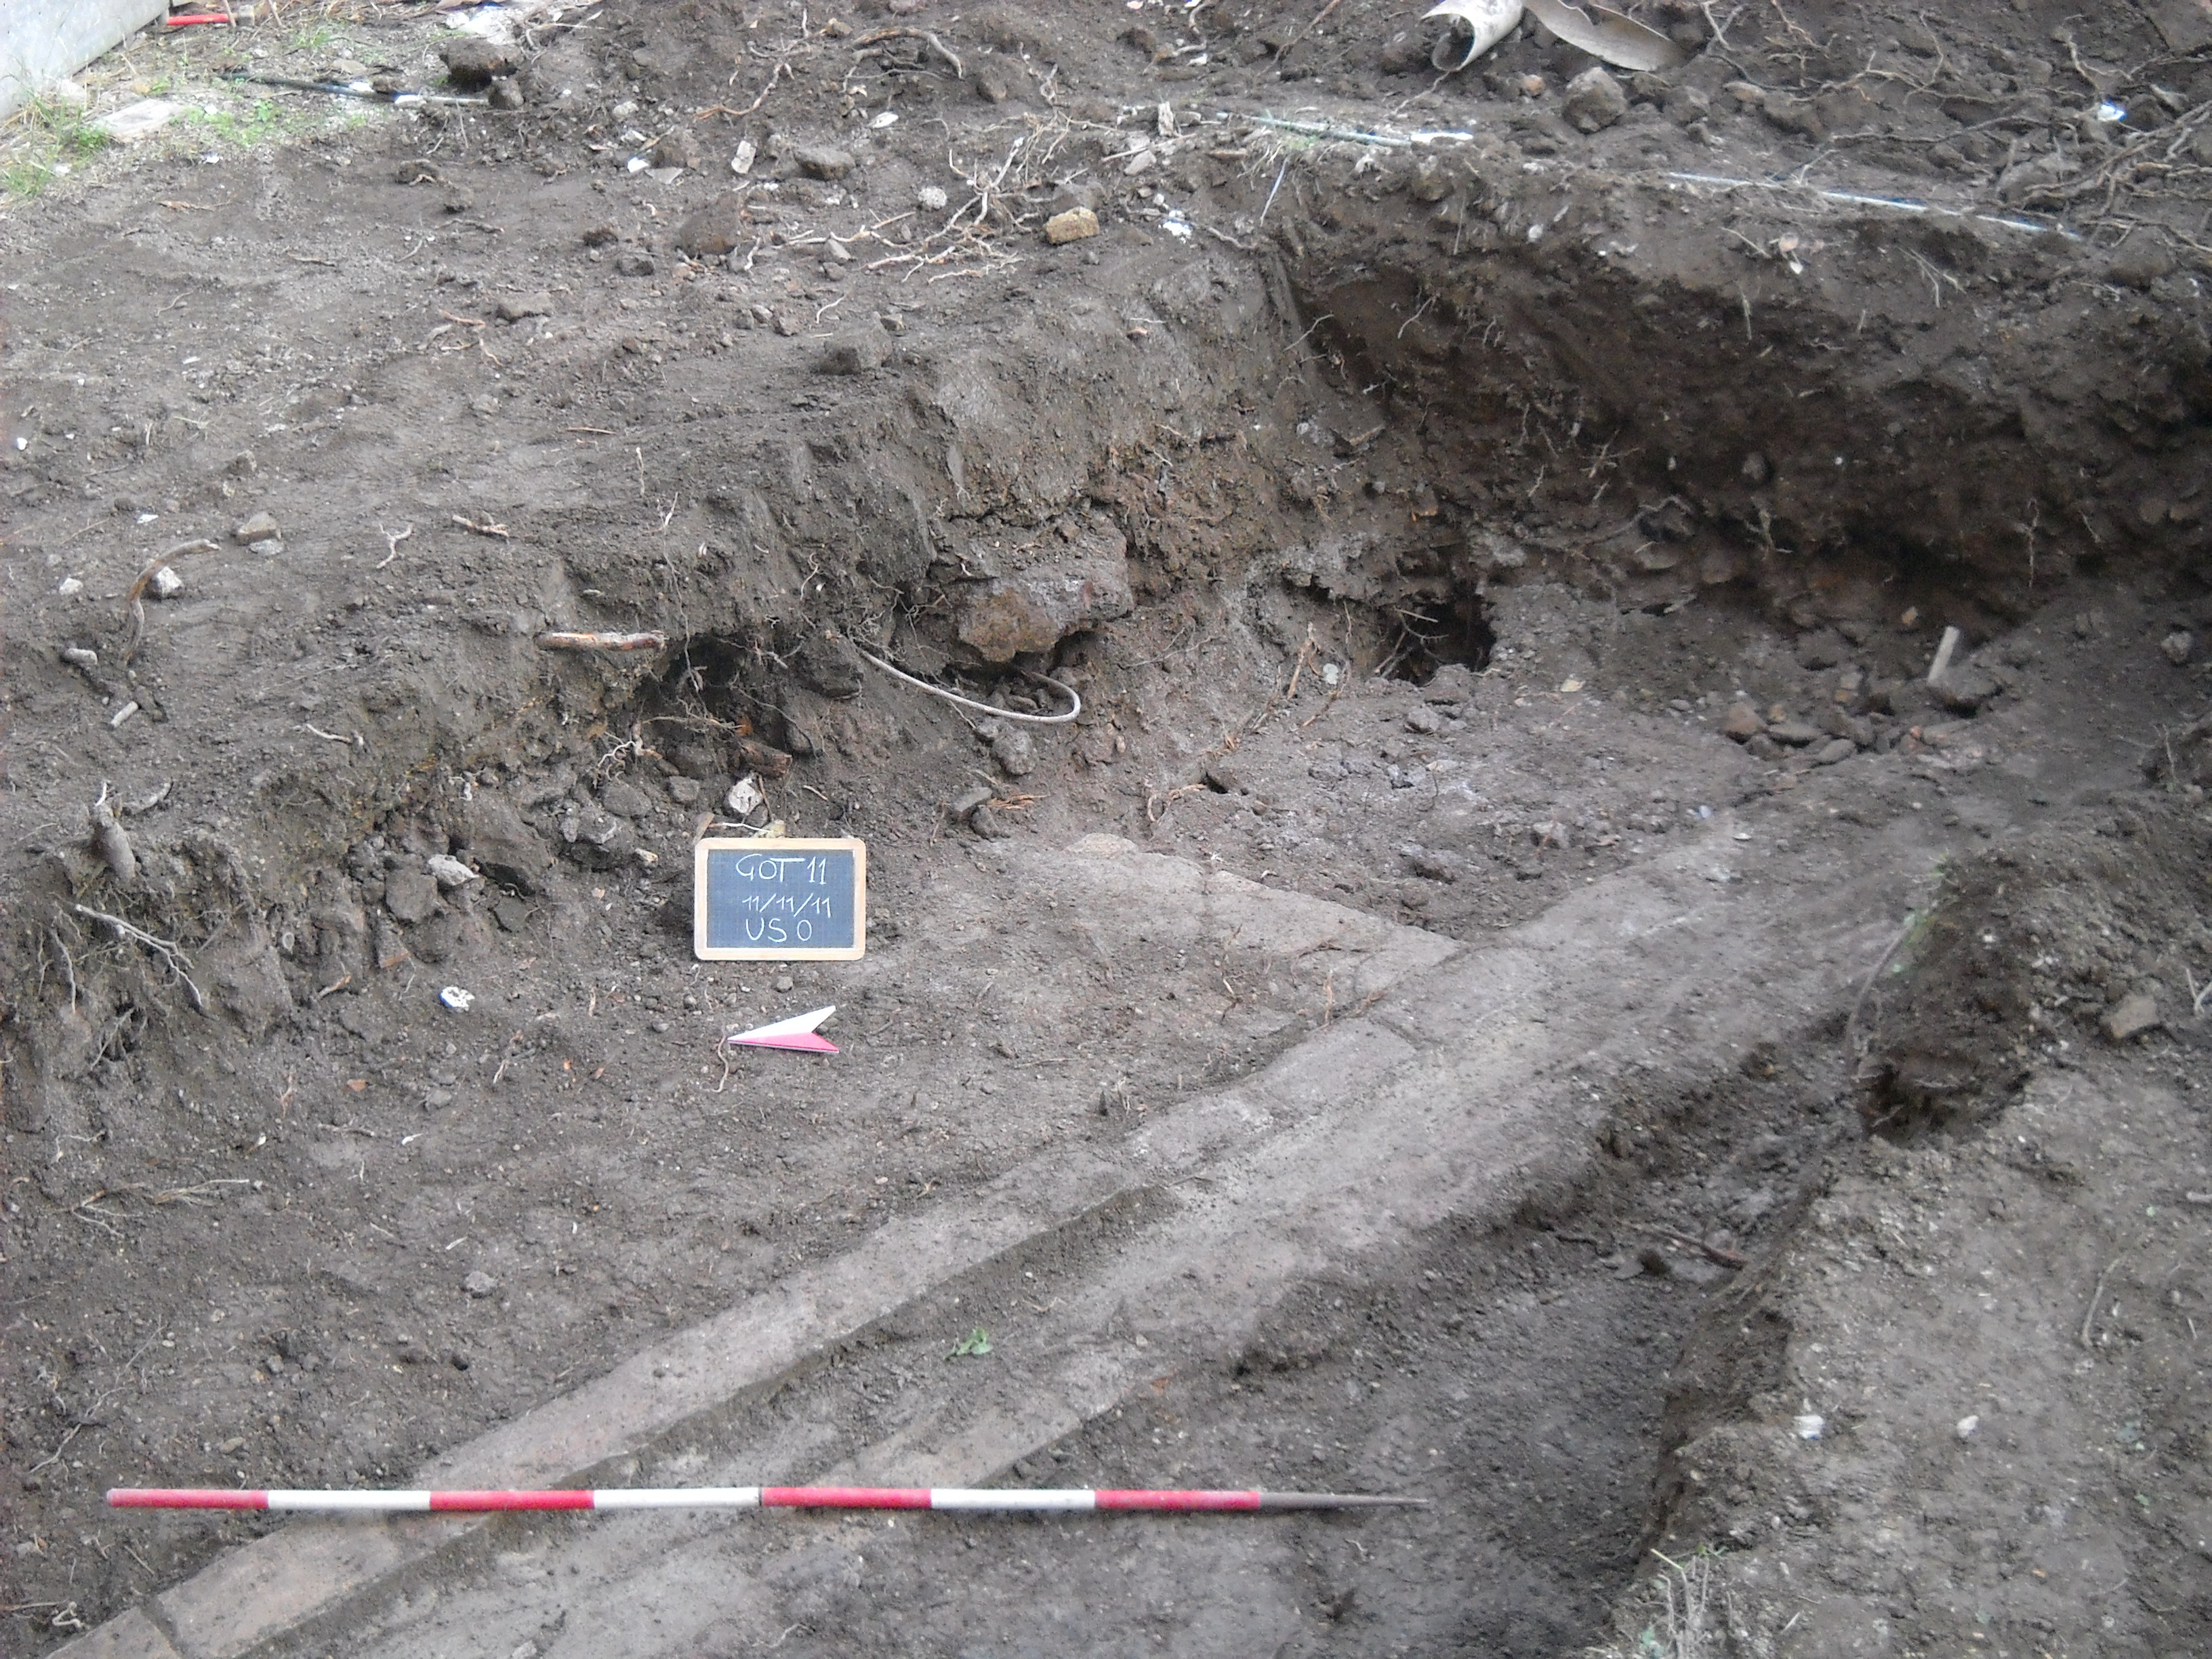
\includegraphics[width =0.5\textwidth]{catacom_1020.JPG}
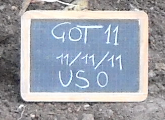
\includegraphics[width=0.5\textwidth]{catacom_1020_cutout.png}
\caption{Beispiel eines Fotos der verwendeten Tafel. GOT bezeichnet die Kampagne, darunter folgt das Datum. US ist die Abkürzung für \textit{unità stratigrafica}, die stratigrafische Einheit.}
\label{fig:einfachetafel}
\end{figure}
Die im Beispielbild gezeigte Tafel stellt  ein Idealbild dar: Die Tafel nimmt einen relativ großen Teil des Originalbildes ein. Sie ist frontal vor der Kamera positioniert. Die Beleuchtung ist gut und indirekt. Keines der weiteren Bildelemente verdeckt die Tafel.
Diese Beschreibung impliziert schon die Problemfelder, die bei der Detektion beachtet werden müssen:
\begin{enumerate}
\item Die Tafel ist unter Umständen stark rotiert (Vgl. Abb \ref{fig:schwierigetafel}).
\item Die Distanz der Tafel zur Kamera und damit ihre Größe im Bild kann stark variieren.
\item Der Rahmen der Tafel kann teilweise verdeckt oder anderweitig durch Gegenstände überlagert sein (Vgl. Abb \ref{fig:schwierigetafel}).
\item Die Farbe des Tafelrahmens kann dazu führen, dass sie sich nicht klar vom Hintergrund abhebt, was die Detektion des (äußeren) Randes erschweren kann.
\item Unregelmäßigkeiten im Rahmen, die auf grobe Verarbeitung oder Abnutzung zurückzuführen sind, können die Detektion erschweren.
\item Die Beleuchtung kann zu Problemen führen. Grundsätzlich sind alle Fotos hell und gut ausgeleuchtet, direktes Licht kann sich aber negativ auf die Kontraste auswirken.
\item Weitere Gegenstände, die den Spezifika der Tafeln entsprechen, können im Bild vorhanden sein.
\end{enumerate}
\begin{figure}[!h]
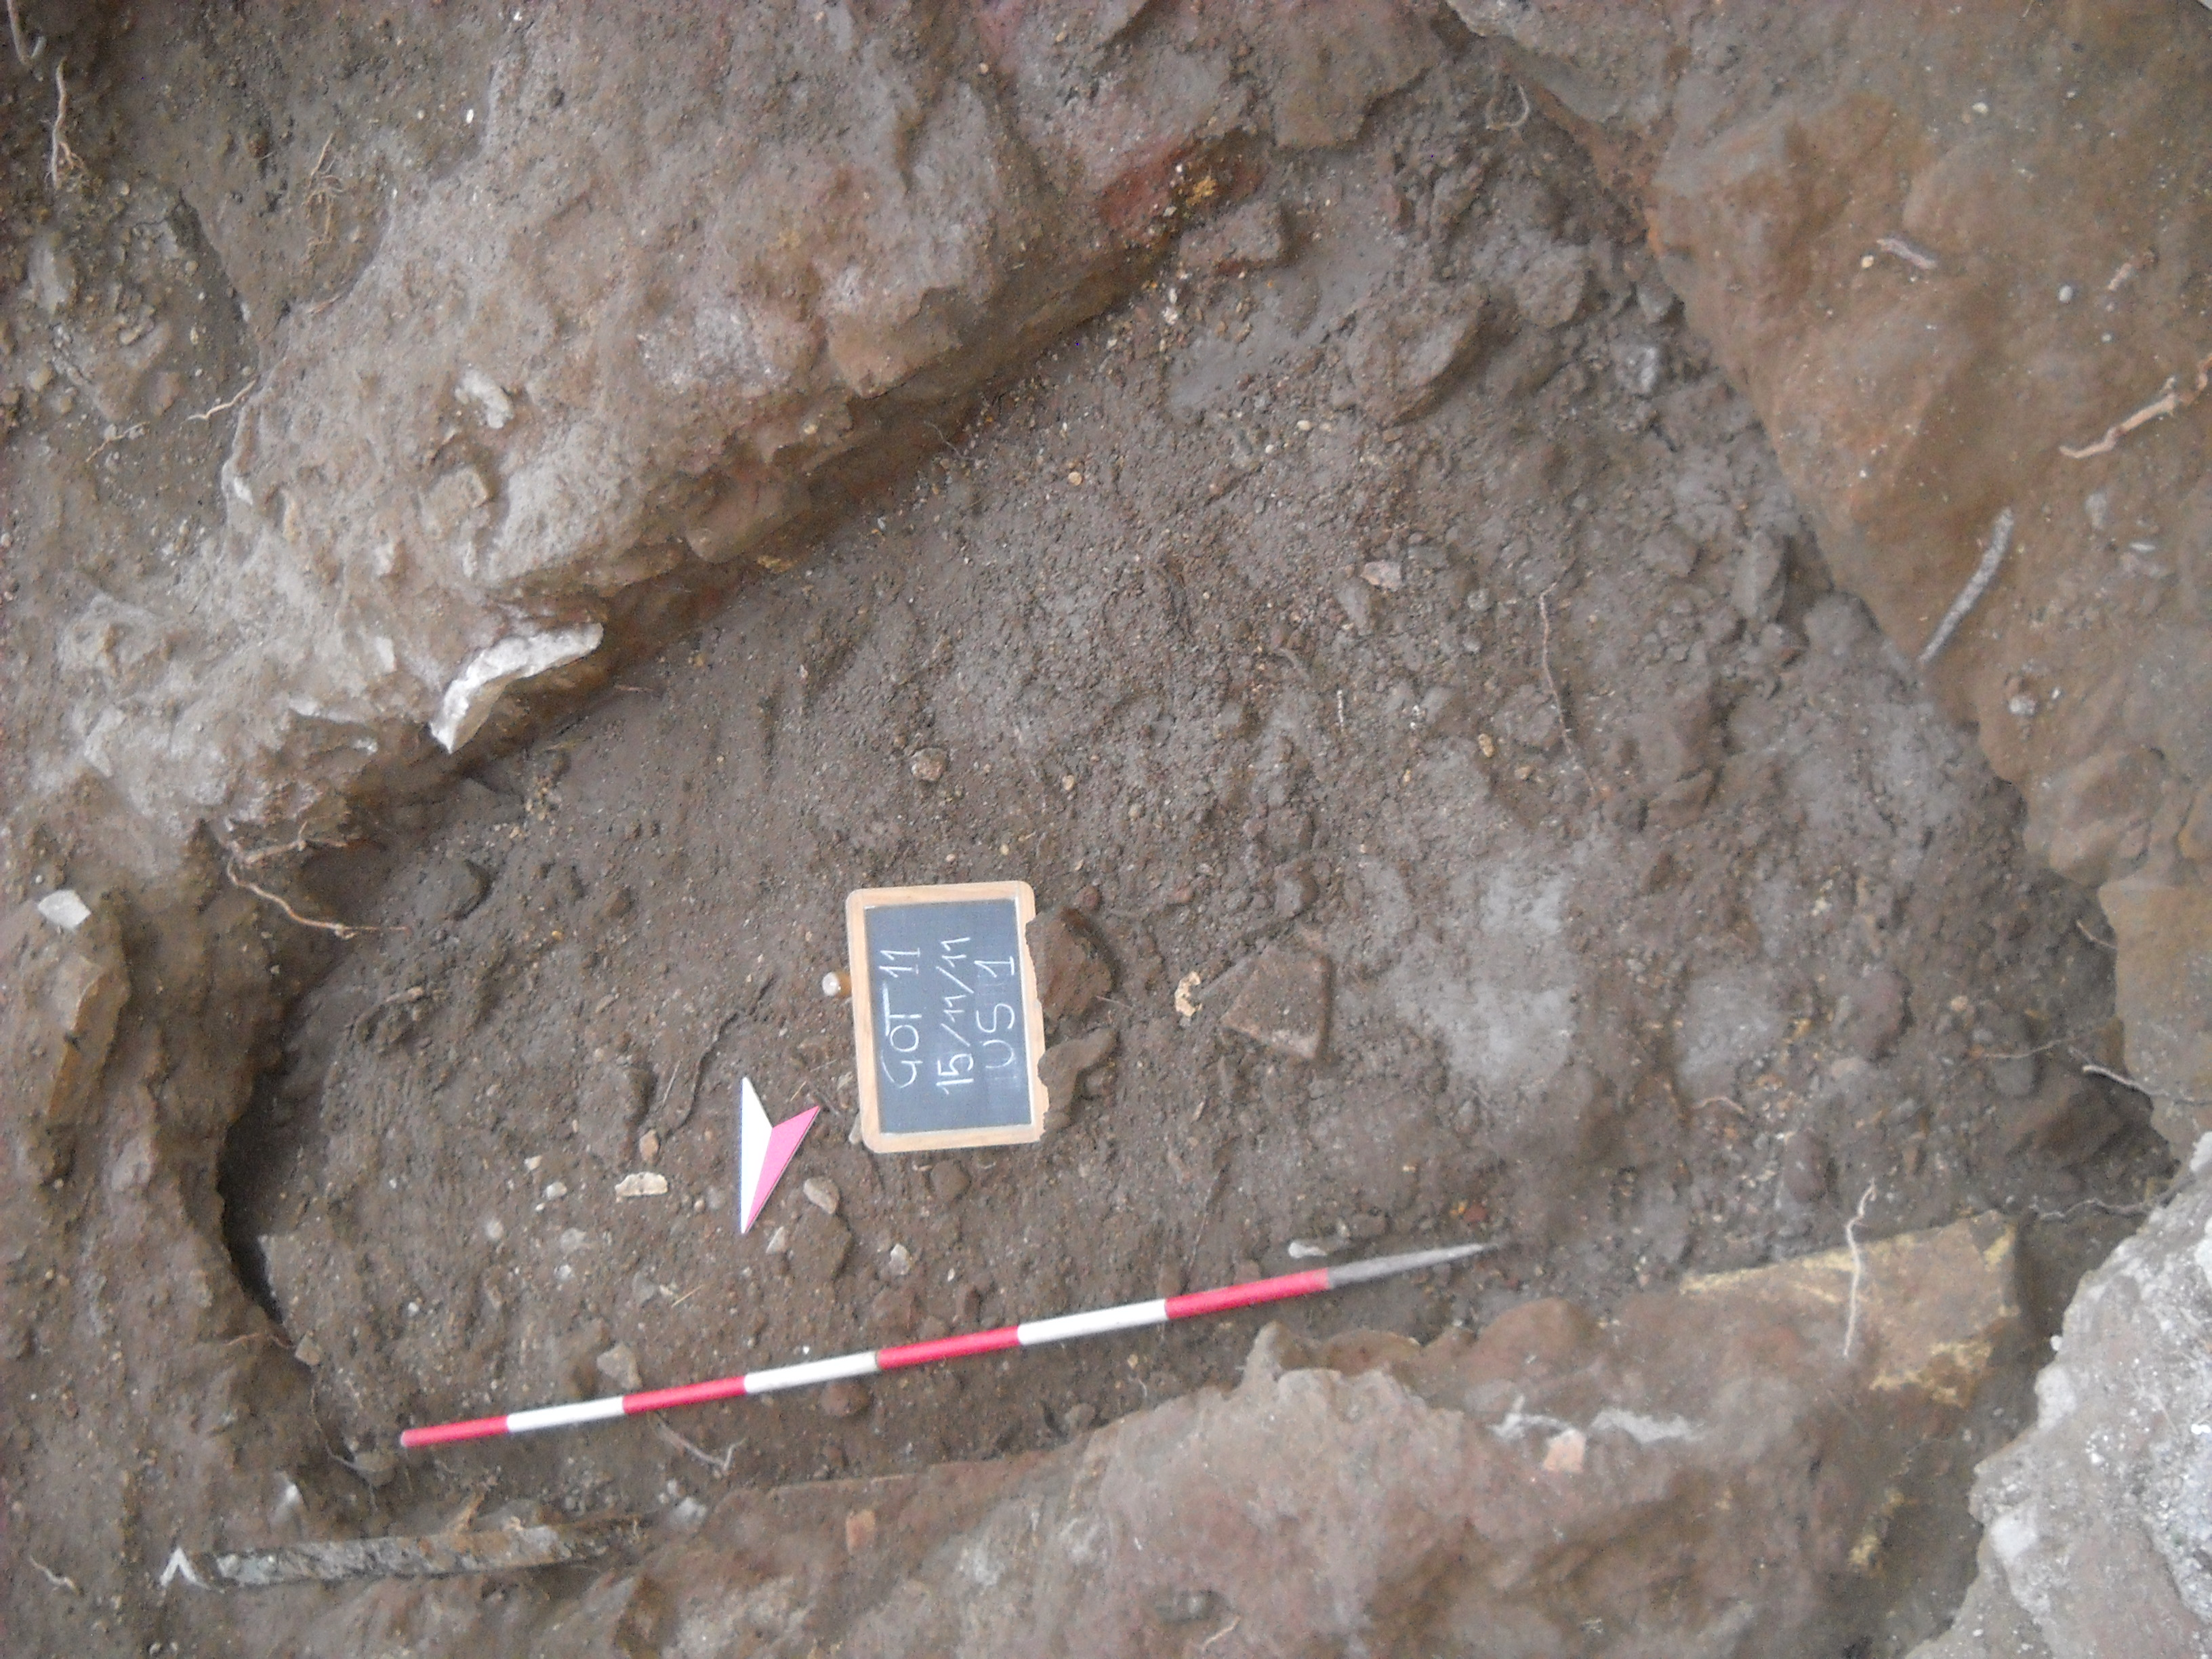
\includegraphics[width =0.5\textwidth]{catacom_1061_schwierige_tafel.JPG}
\caption{Schwierigere Detektion: Rotation und teilweise verdeckter Rahmen.}
\label{fig:schwierigetafel}
\end{figure}
Teilweise werden die hier genannten Probleme auch bei der Texterkennung wieder relevant. Auf diese und auf weitere wird an geeigneter Stelle zurückgegriffen.


\subsubsection{Tafelvergleiche}

Im Rahmen der Arbeit wurden weitere Tafeln exemplarisch dem Algorithmus unterzogen. Dabei handelte es sich um Aufnahmen der späteren Grabungen des Deutschen Archäologischen Institutes am Kapitol in Rom sowie um vergleichbare Fotos von Bodenuntersuchungen der Gruppe Terrestrische Ökohydrologie der Friedrich-Schiller-Universität Jena. Der ursprüngliche Gedanke dahinter war eine möglichst universale Detektion von Tafeln aller Art anzustreben. Die unterschiedlichen Daten konnten dabei vor allem Stärken und Schwächen der letztlich gewählten Technik aufzeigen.\\
Die Tafeln beider Projekte sollen im Folgenden kurz vorgestellt werden, um das Spektrum der Komplexität 
evtl. Vergleiche zu Tafeln aus späterer Grabung als Positivbeispiel:\\
besser gearbeitete Tafeln\\
besser lesbare Schrift\\
evtl. Vergleiche zu Tafeln der Bodenkunde als Negativbeispiel:\\
Tafel schwierig durch Form und Farbe\\
Klarsichthülle: Reflektion und Formveränderung\\
oft verdeckt\\
Bilder zur Veranschaulichung einfügen

\subsubsection{Schrift}
Kreide auf Schiefer
Probleme wie Handschrift, Verwischung, Karomuster
\subsection{Pipeline}
Struktur der Arbeit wie Pipeline:
Bildakquise
Objekterkennung
Crop-Verfahren
Pre-Processing
OCR
Evaluation
Ergebnis
%\section{Theorie}


\section{Material und Methoden}

In diesem Kapitel werden das zu Grunde liegende Material -- die Grabungsfotos -- und die darauf angewendete Software vorgestellt. Außerdem wird die Verarbeitung der Fotos im Detail beschrieben. 
Diese gliedert sich in zwei Teilbereiche: Die Tafeldetektion und die Texterkennung (OCR). Die Tafeldetektion wiederum ist in die eigentliche Erkennung sowie das Ausschneiden der Tafeln aus dem Gesamtbild unterteilt. Für beide Arbeitsschritte gibt es je zwei Varianten.
%eigentliches Material: Fotos!
\subsection{Fotos}
Der Gegenstand dieser Arbeit sind 1.424 Fotos, die während der Grabungen auf dem Kapitol in Rom in den Jahren 2011-2014 entstanden sind. Die Fotos haben eine Auflösung von 3264 x 2448 Pixeln und liegen im JPG-Format vor. Teilweise sind die exif-Daten (\textit{Exchangeable Image File Format}) vorhanden, die von der Kamera erzeugt wurden, also Informationen, die nach den Standards für Metadaten in Bilddateien\cite{exif}{} angelegt wurden. Sie beinhalten das Datum, das Kameramodell (Nikon Coolpix L19), die Belichtungsdauer und den ISO-Wert für die Lichtempfindlichkeit des Fotosensors. Weitere Metadaten -- Datum, Ort, das Kürzel für die Grabung sowie weitere Anmerkungen -- befinden sich auf Tafeln, die auf etwa einem Drittel der Fotos zu sehen sind. Das Datum auf der Tafel und das in den exif-Daten weichen teilweise um mehrere Tage voneinander ab. Allerdings sind beide Daten von Bedeutung, um den Grabungsverlauf zu rekonstruieren.
Bei den Tafeln, die auf den Grabungsfotos zu sehen sind, handelt es sich um Schiefertafeln mit einem Holzrahmen, die mit Kreide beschriftet wurden (Abbildung \ref{fig:einfachetafel}). Die Detektion der Tafeln beruht auf folgenden Faktoren: (1) Die Tafeln haben grundsätzlich eine rechteckige Form. (2) Durch die Breite des Rahmens können bis zu zwei Rechtecke erkannt werden, ein inneres und ein äußeres. (3) Der Rahmen ist hell und die Schreibfläche dunkel, es besteht ein starker Kontrast.
\begin{figure}[!h]
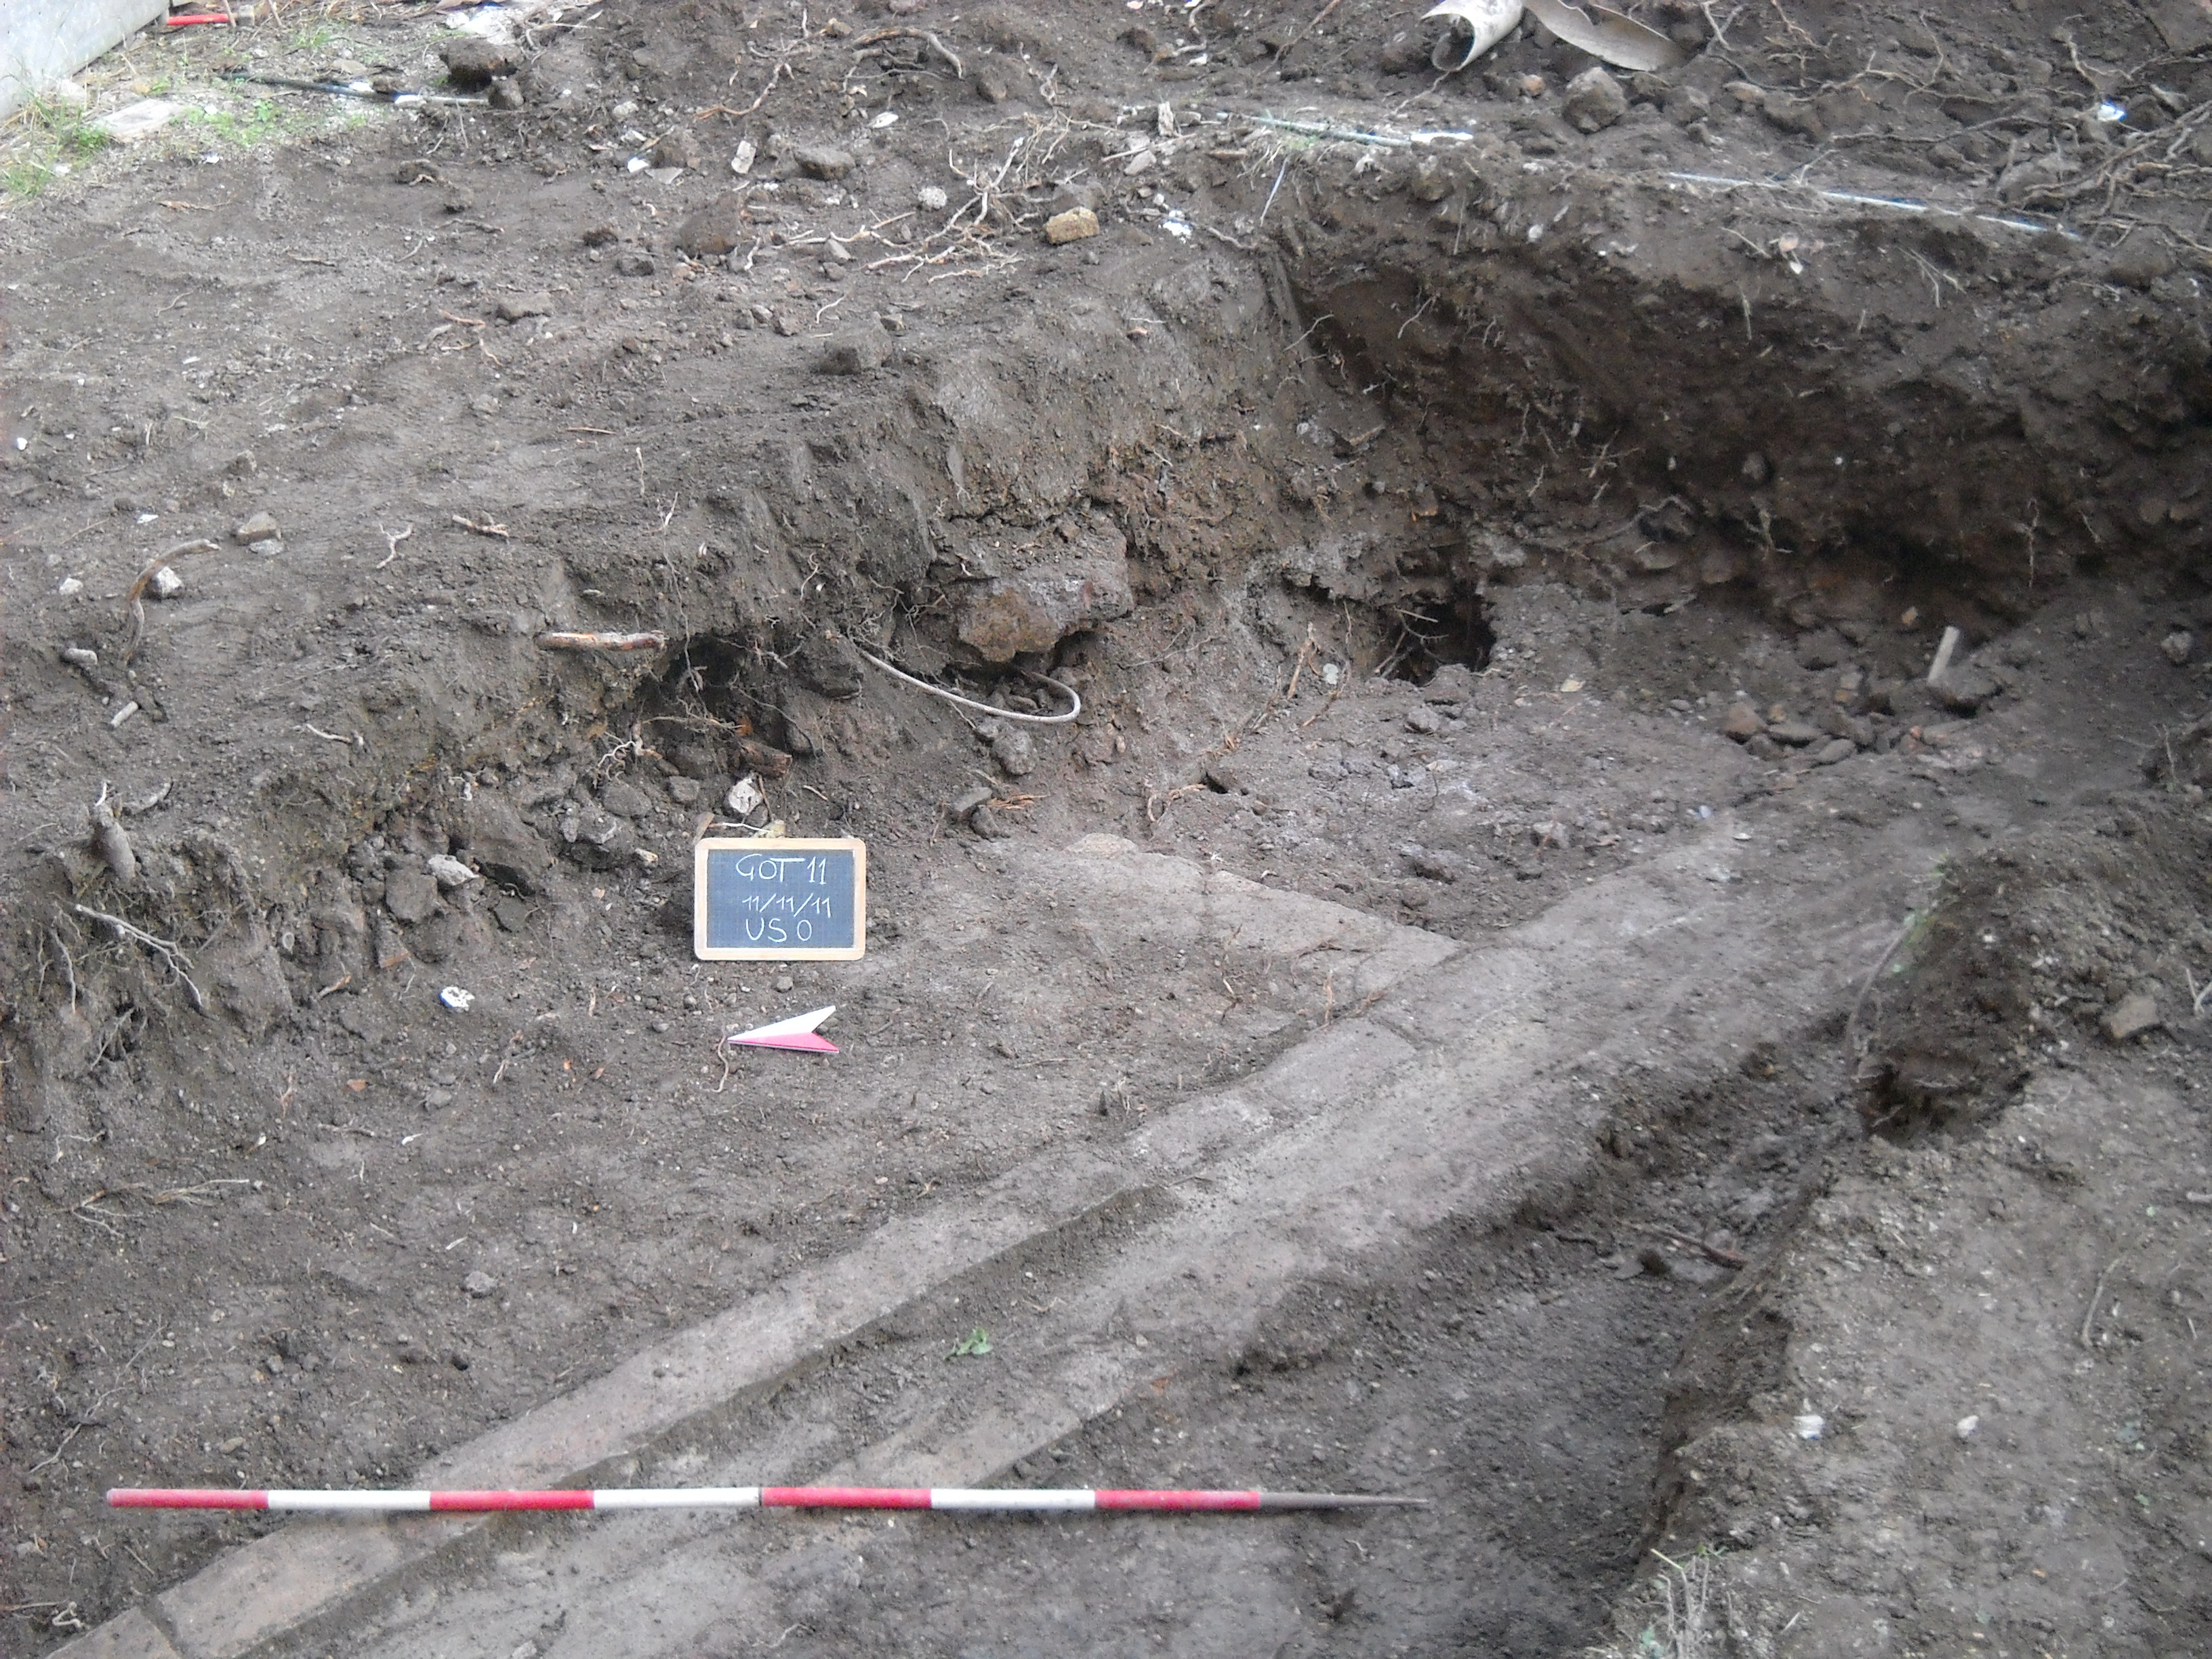
\includegraphics[width =0.5\textwidth]{catacom_1020.JPG}
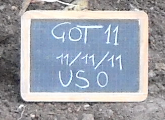
\includegraphics[width=0.5\textwidth]{catacom_1020_cutout.png}
\caption{Beispiel eines Fotos der verwendeten Tafeln. GOT bezeichnet die Kampagne, darunter folgt das Datum. US (\textit{unità stratigrafica}) bezeichnet die stratigrafische Einheit.}
\label{fig:einfachetafel}
\end{figure}
Die im Beispielbild gezeigte Tafel stellt  ein Idealbild dar: Die Tafel nimmt einen relativ großen Teil des Originalbildes ein. Sie ist frontal vor der Kamera positioniert. Die Beleuchtung ist gut und indirekt. Keines der weiteren Bildelemente verdeckt die Tafel.
Diese Beschreibung impliziert schon die Problemfelder, die bei der Detektion beachtet werden müssen:
\begin{enumerate}
\item Die Tafel ist unter Umständen rotiert (Abbildung \ref{fig:schwierigetafel}).
\item Die Distanz der Tafel zur Kamera und damit ihre Größe im Bild kann stark variieren.
\item Der Rahmen der Tafel kann teilweise verdeckt oder anderweitig durch Gegenstände überlagert sein (Abbildung \ref{fig:schwierigetafel}).
\item Ein geringer Kontrast des Hintergrunds zum Tafelrahmen kann die Detektion erschweren. %(Vgl. Abb \ref{fig:schwierigetafel})
\item Unregelmäßigkeiten im Rahmen, die auf grobe Verarbeitung oder Abnutzung zurückzuführen sind, können die Detektion erschweren.
\item Die Beleuchtung kann zu Problemen führen. Grundsätzlich sind alle Fotos hell und gut ausgeleuchtet, direktes Licht kann sich aber, bedingt durch Spiegelungen, negativ auf die Kontraste auswirken.
\item Weitere Gegenstände, die den Spezifika der Tafeln entsprechen, können im Bild vorhanden sein.
\end{enumerate}
\begin{figure}[!h]
\centering
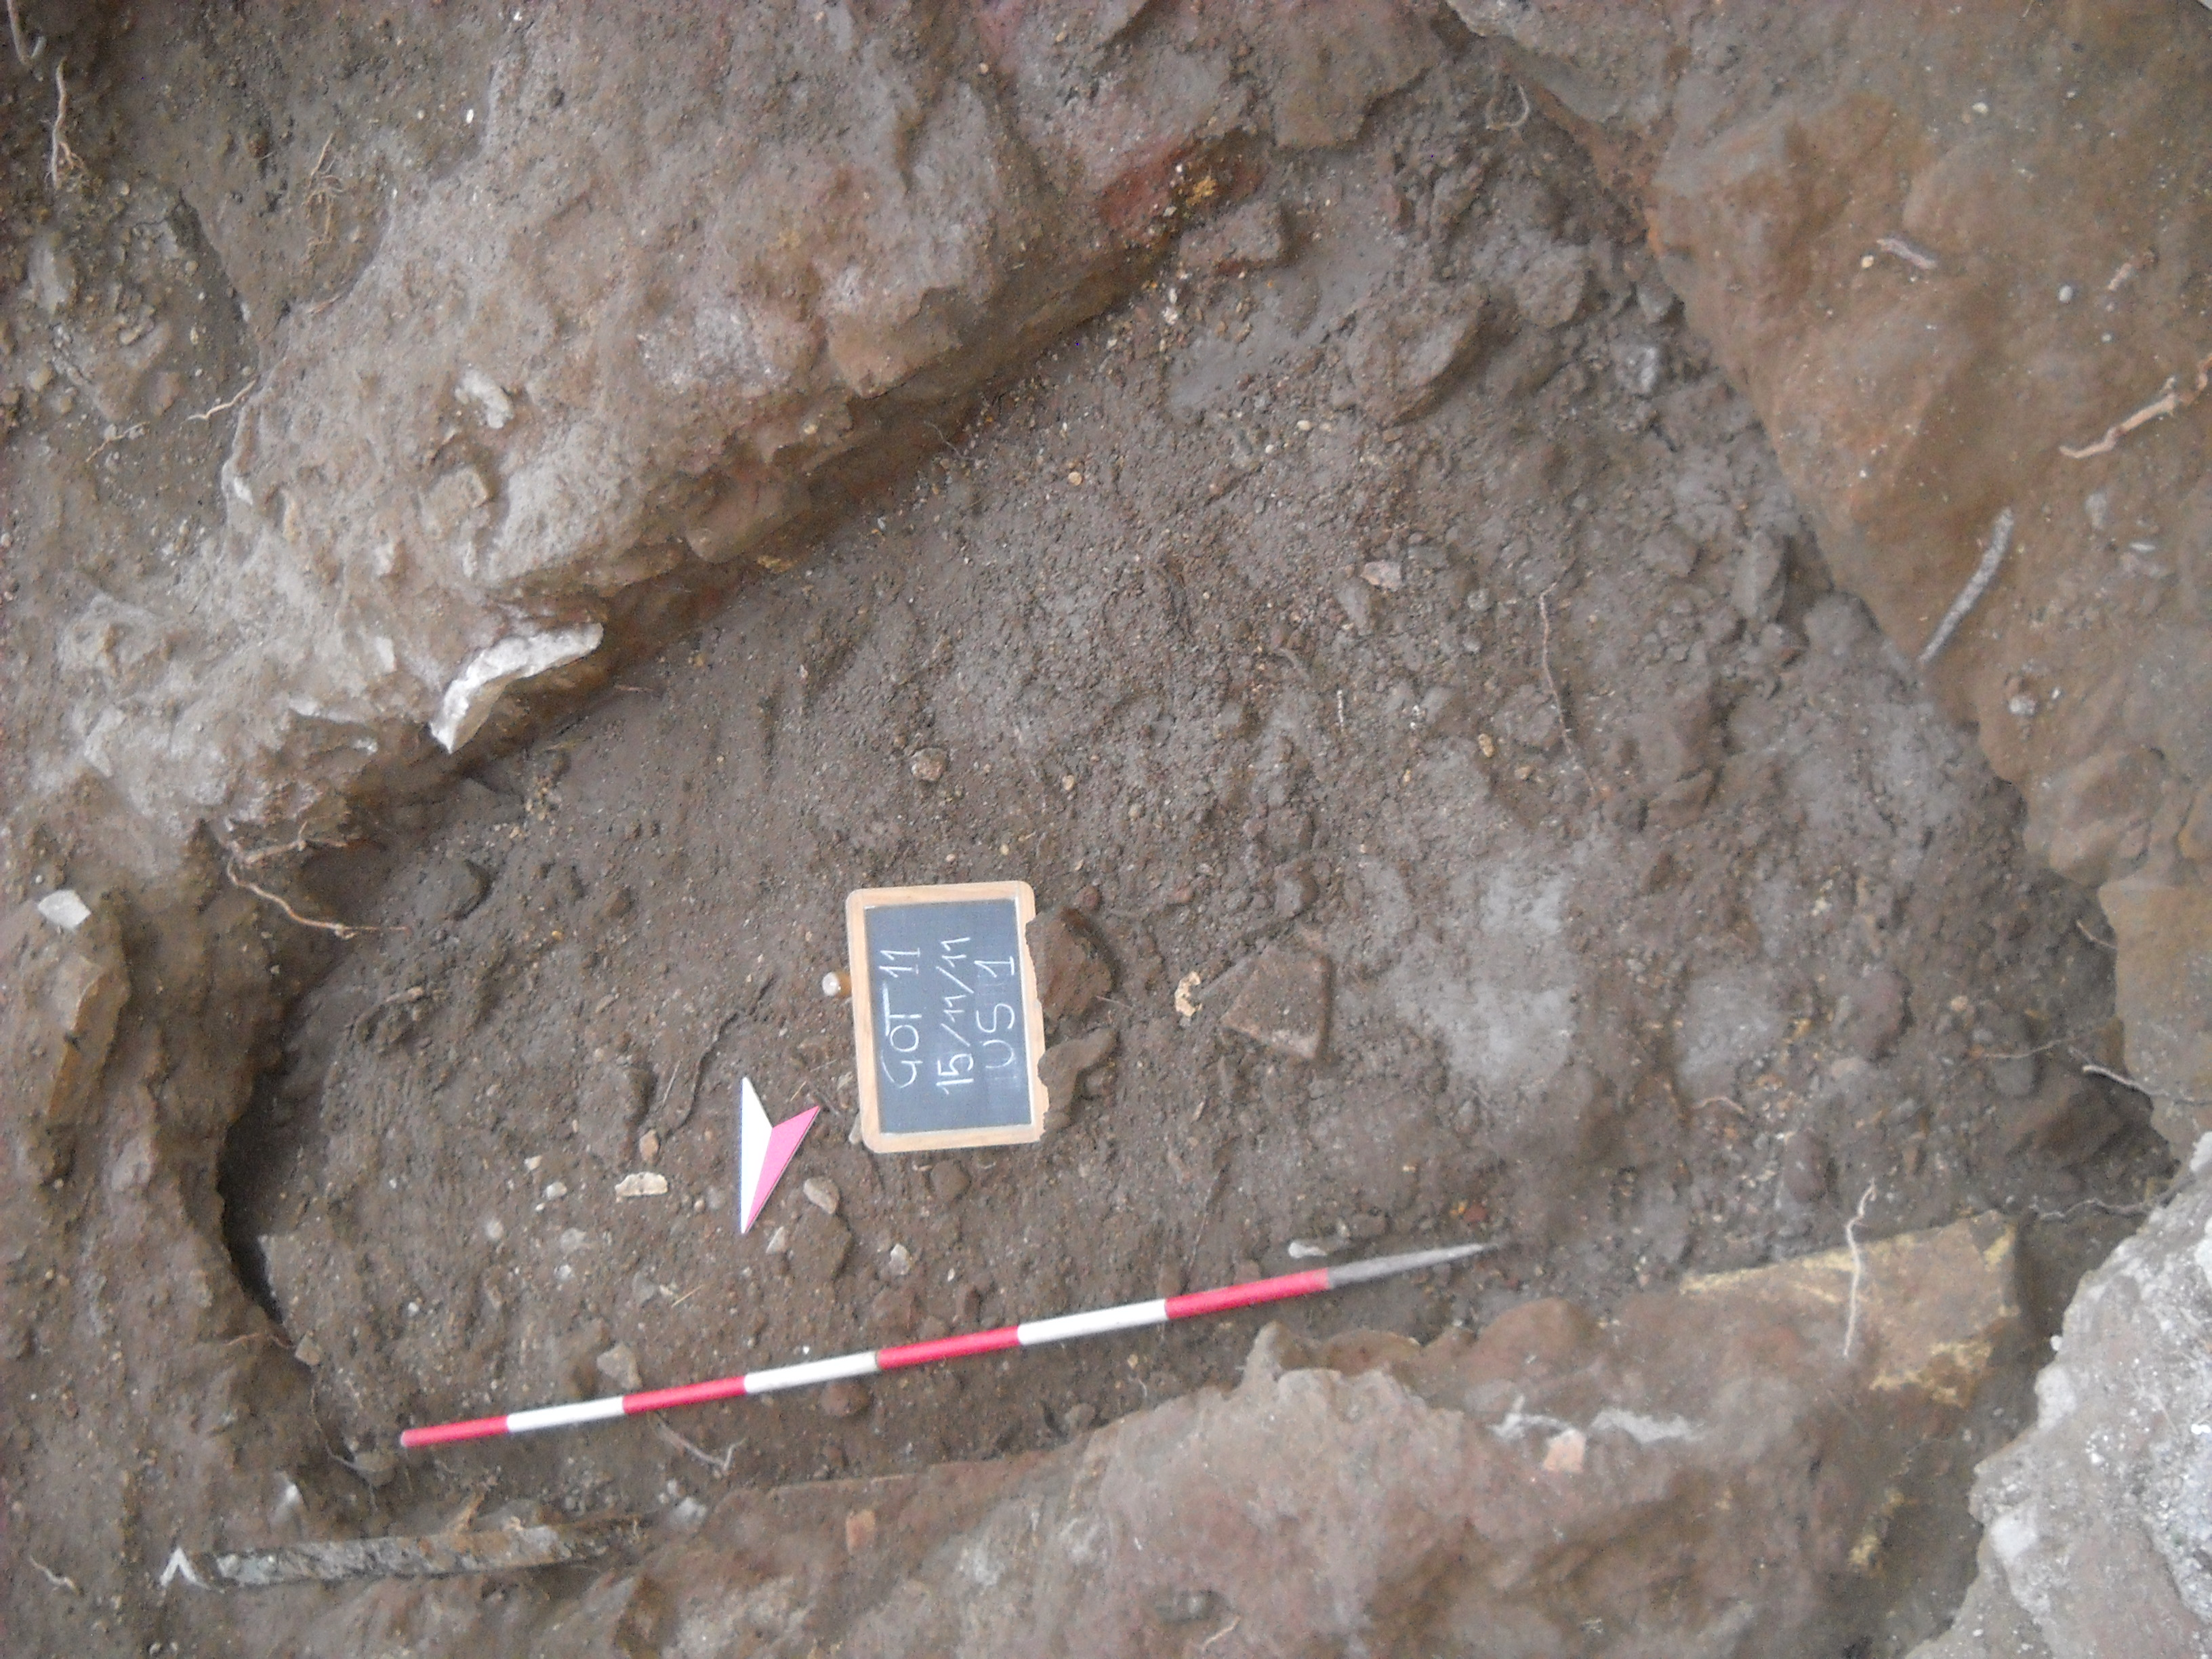
\includegraphics[width =0.5\textwidth]{catacom_1061_schwierige_tafel.JPG}
%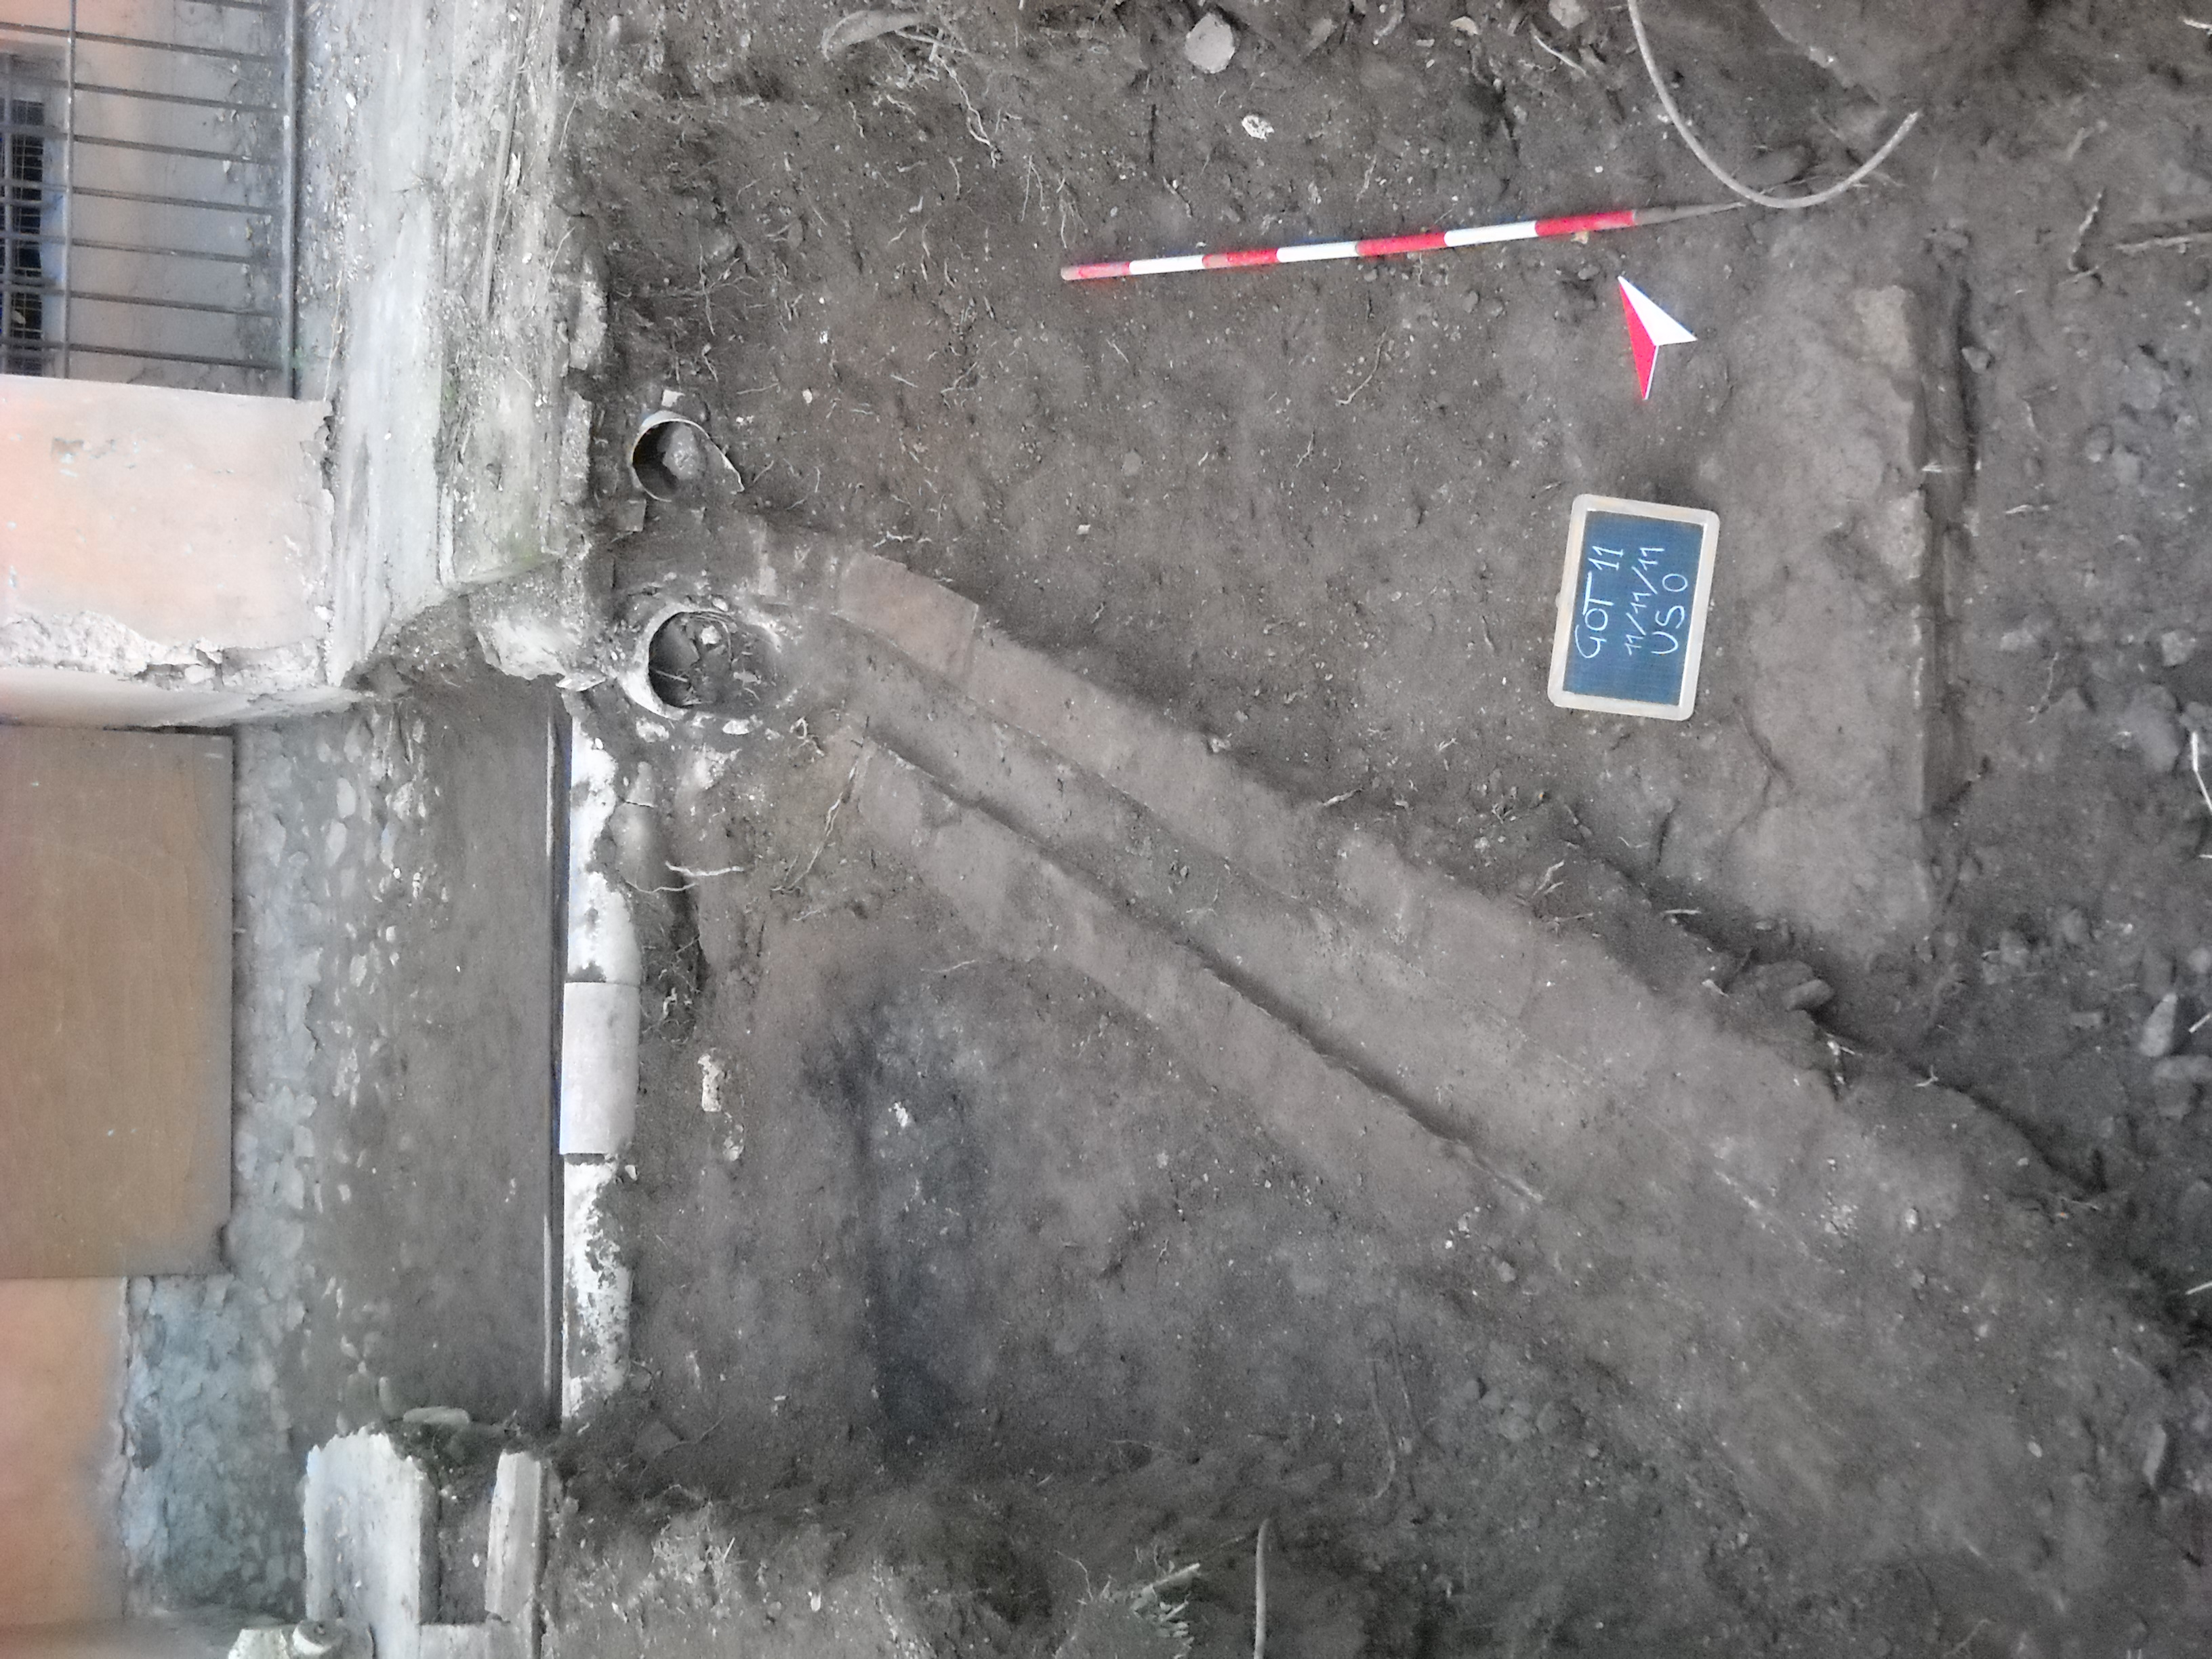
\includegraphics[width =0.5\textwidth]{catacom_1023.JPG}
\caption{Problematische Tafeln: Rotation und teilweise verdeckter Rahmen.}
\label{fig:schwierigetafel}
\end{figure}
%Teilweise werden die hier genannten Probleme auch bei der Texterkennung wieder relevant. Auf diese und auf weitere wird an geeigneter Stelle zurückgegriffen.

\subsection{Software}

Der Programmcode ist in Python (Version 3.8) geschrieben. Grund für diese Wahl war, dass sowohl OpenCV als auch verschiedene OCR-Engines über Python-Anbindungen verfügen. Verwendet werden die \textit{packages} Numpy (1.19.5) und vor allem OpenCV (4.4.0.44). Die Texterkennung arbeitet mit PyTesseract (0.3.7). Für die Evaluation wurde die Bibliothek Difflib (3.8) eingebunden.

\subsection{Tafeldetektion}

Der folgende Abschnitt befasst sich mit der ersten Teilaufgabe dieser Arbeit: Der Detektion der Tafeln auf den Grabungsfotos. Hier werden mehrere Ansätze vorgestellt, die im Laufe der Auseinandersetzung mit dem Thema erprobt wurden: die Tafeldetektion mittels CNNs und mittels klassischer Computer Vision über die Detektion von Konturen.

\subsubsection{CNN-basierter Ansatz}

Der auf Convolutional Neural Networks (CNN) basierende Ansatz bestand darin, bereits bestehende, trainierte Datensätze für die Bilderkennung auf die Grabungsfotos anzuwenden.\\
CNNs werden auf großen Datenbanken mit bekannten Klassifizierungen trainiert, um unbekannte Bilder auf dieser Grundlage klassifizieren zu können. So basiert das COCO-Dataset\footnote{Common Objects in Context \cite{coco}.} auf über 330.000 Bildern mit 1,5 Millionen Objekten darauf \cite{coco}. Das Training wird, je nach Datenmenge, auf dafür geeigneten Grafikkarten oder Großrechnern durchgeführt \cite{ki}.\\
Da die  Tafeln Objekten wie Büchern, Verpackungen von Frühstücksflocken oder anderen rechteckigen, beschriebenen Objekten ähneln, die im trainierten Datensatz enthalten sind, sollte hier geprüft werden, ob die Tafeln regelmäßig und zuverlässig als eines dieser Objekte erkannt werden.
%CNNs machen Muster in Bildern erkennbar, indem sie Bilder mithilfe von Kernels, durch die eine Gewichtung vorgenommen wird, mathematisch falten (\textit{convolute}). Die Ergebnisse werden durch \textit{Pooling} in der Größe reduziert. Die beiden Prozesse werden wiederholt, bis der gewünschte Komplexitätsgrad erreicht ist. Das Ergebnis in einem oder mehreren Fully-connected Layern ausgewertet, in denen Neuronen aktiviert werden, wenn bestimmte Schwellwerte überschritten werden \cite{introduction}. Im Ergebnis kann das CNN vorher trainierte, komplexe Muster erkennen.
Zum Einsatz kamen auf dem Datensatz von COCO trainierte Modelle mit Gewichten von COCO und YOLO (You Only Look Once \cite{yolo}{} \cite{yolo2}).


\subsubsection{Kontur-basierter Ansatz}

Beim Kontur-basierten Ansatz wurden die Umrisse der Objekte auf dem Foto erfasst. Aus diesen sollten alle Objekte mit annähernd rechteckiger Form ausgewählt werden. Bei diesen, so die Annahme, handelt es sich um mögliche Tafeln.\\
\verb|Cv2.Contours| basiert auf einem Algorithmus, der Punkte gleicher Farbe und Intensität umrandet \cite{findcontours}. Das Resultat ist eine Liste von Punkten, die ein geschlossenes Polygon ergeben. Die gefundenen Konturen können mit einer Hierarchie versehen werden: Konturen, die sich innerhalb anderer Konturen befinden, gelten als deren \glqq Kinder\grqq. Das Verfahren ist darauf ausgelegt, auf binäre Bilder angewendet zu werden. Die Implementierung in OpenCV unterscheidet in Nullwerte und Nicht-Nullwerte \cite{opencvcontours}. Nicht-binäre Bilder werden dadurch automatisch binarisiert. Für die Erzielung optimaler Ergebnisse kommt dem Binarisierungsverfahren eine große Bedeutung zu.\\
Auf Basis dieses Algorithmus lässt sich Detektionsverfahren aufbauen, das Objekte, die sich vom Hintergrund der Bilder abheben, erkennt. Die Herausforderung bestand, nach diesem Ansatz, in zwei Punkten: Erstens musste die Binarisierung so erfolgen, dass eine möglichst saubere Trennung von Vordergrund (Objekten) und Hintergrund (vor allem Erde) der Bilder stattfand und zweitens mussten aus den gefundenen Vordergrundobjekten diejenigen ausgewählt werden, die als Tafeln in Frage kamen. Bei der Binarisierung stellten sich zwei Wege als praktikabel heraus, die hier beide präsentiert werden sollen. Diese Ansätze werden im Folgenden als adaptiver und als iterativer Ansatz bezeichnet. Im Flowchart sind die Abläufe der Rechtecksdetektion dargestellt (Abbildung \ref{fig:flowrectdetect}).
\begin{figure}[h!]
\centering
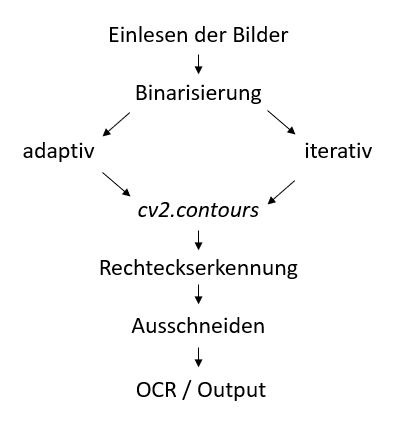
\includegraphics[width =0.5\textwidth]{flowchart_cont.PNG}
\caption{Flowchart Rechteckserkennung: Die Binarisierung erfolgt durch einen der beiden möglichen Ansätze. Auf dieser Basis wird eine Konturerkennung durchgeführt. Aus diesen Konturen werden die Rechtecke ausgewählt und aus dem Gesamtbild ausgeschnitten. Es folgt die weitere Verarbeitung.}
\label{fig:flowrectdetect}
\end{figure}

\subsubsection*{Adaptive Binarisierung}

Das einfachste Verfahren der Binarisierung eines Bildes besteht darin, einen Schwellwert festzulegen. Dieser muss auf der Spanne der Farbwerte, also zwischen 0 und 255, liegen.  Farbwerte unterhalb dieses Schwellwertes werden zu Nullen, Farbwerte darüber zu Einsen. Das Ergebnis ist ein Schwarz-Weiß-Bild. Bei komplexen Szenen, wie den Grabungsfotos, ist dieses Verfahren jedoch zu einfach. So kann ein Foto beispielsweise stark unterschiedliche Beleuchtung, wie direktes Sonnenlicht und Schatten, enthalten. Eine Differenzierung innerhalb dieser Zonen ist so nicht möglich (Abbildung \ref{fig:threshold}).\\
\begin{figure}[h!]
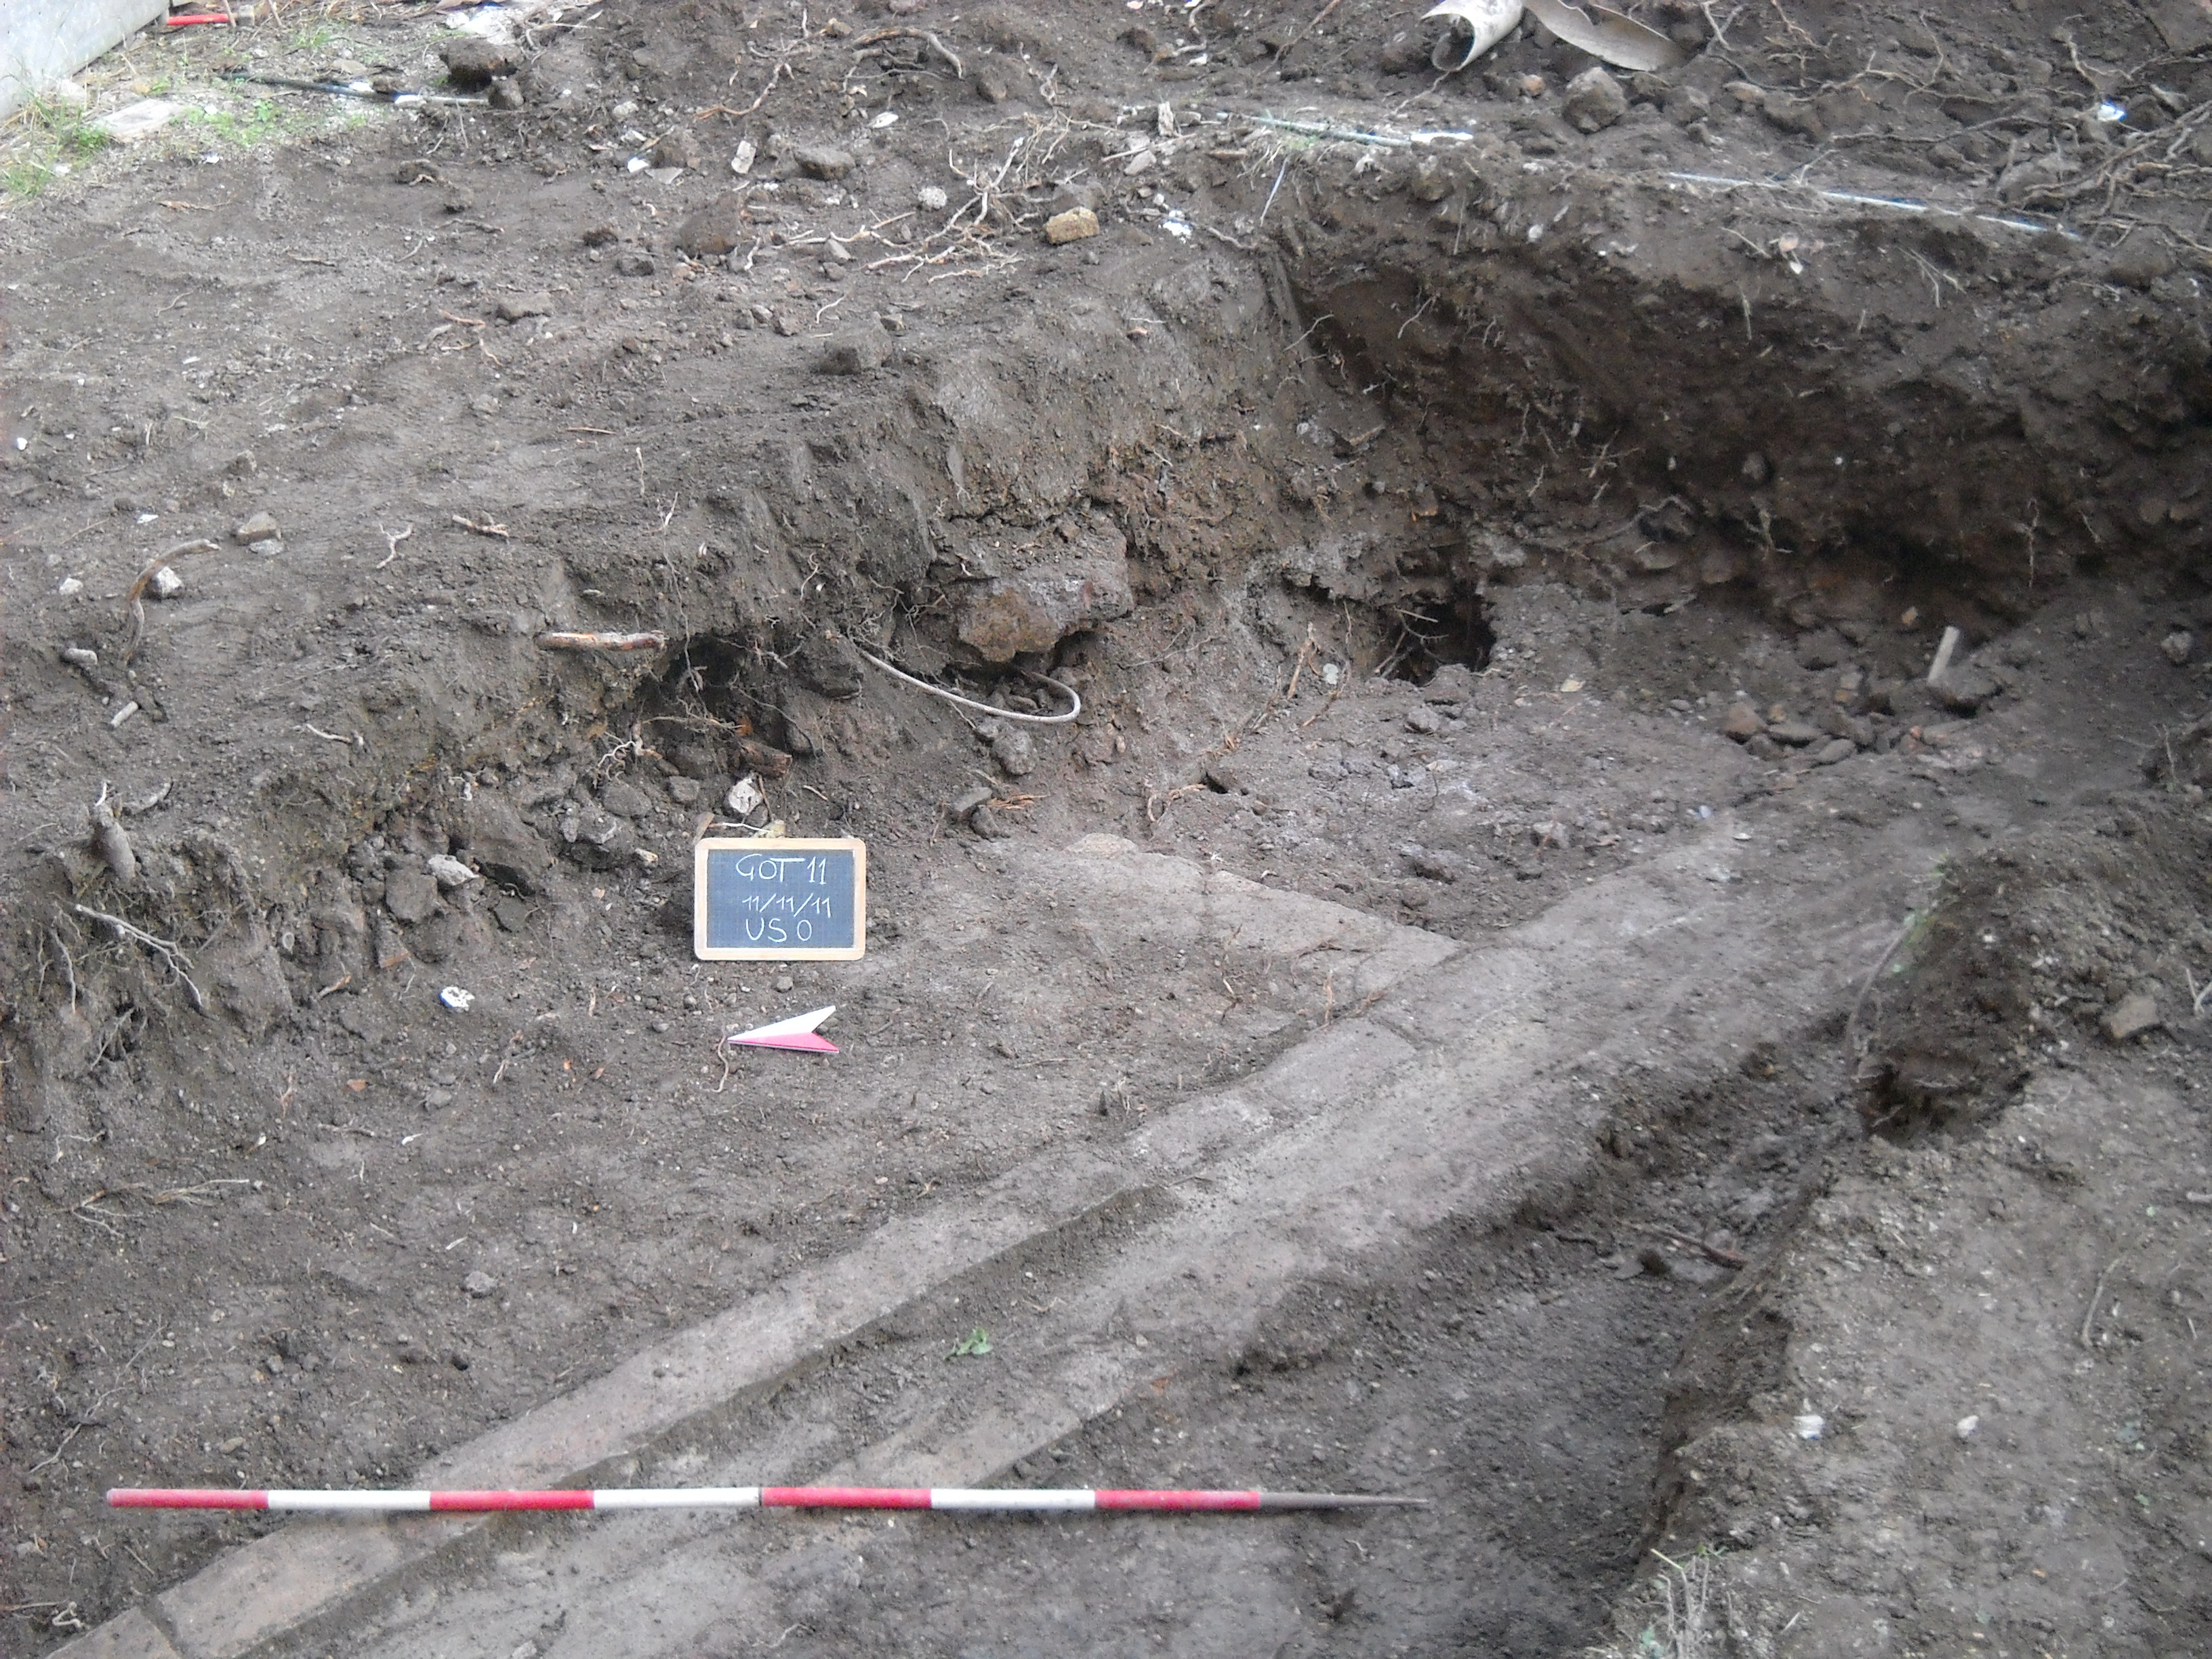
\includegraphics[width =0.5\textwidth]{catacom_1020.JPG}
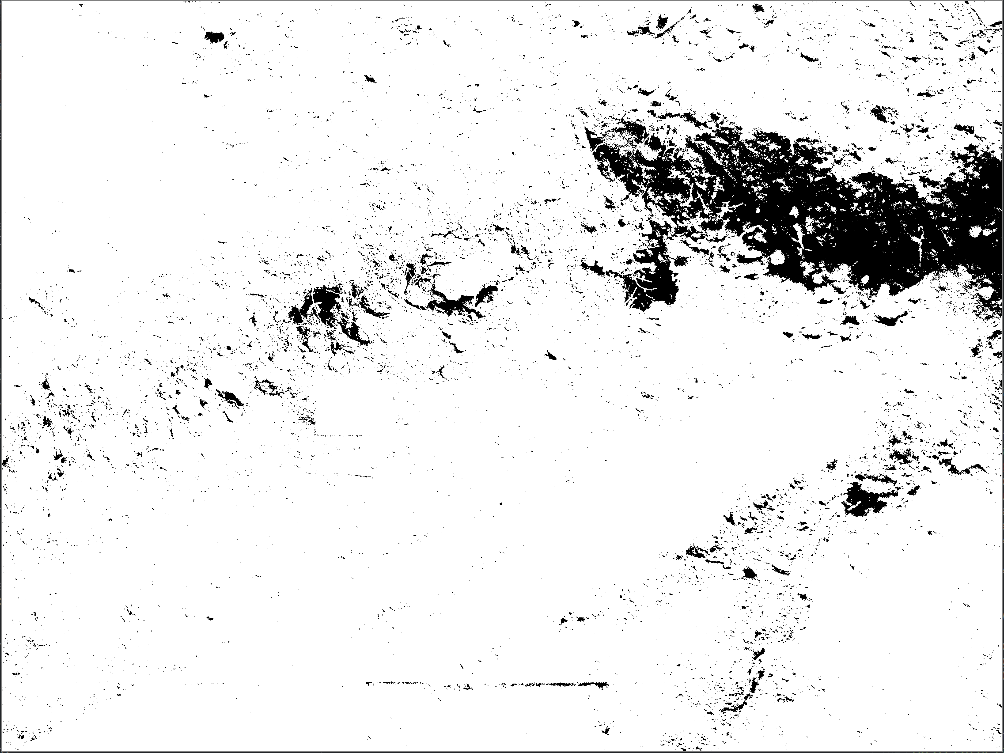
\includegraphics[width =0.5\textwidth]{thresh60.png}
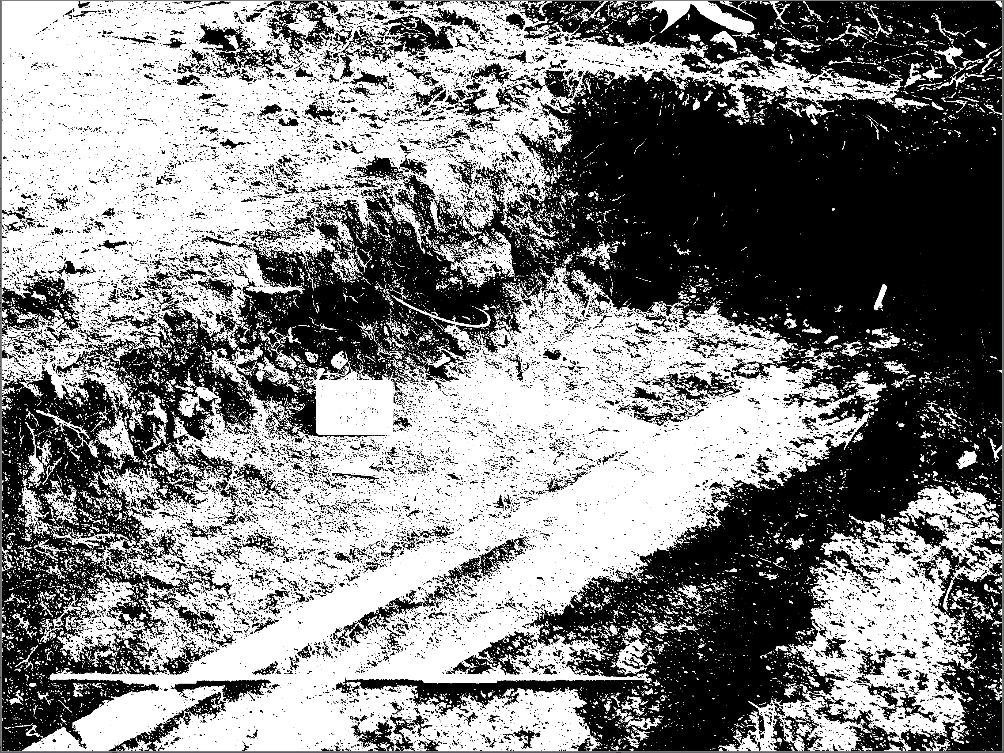
\includegraphics[width =0.5\textwidth]{thresh125.png}
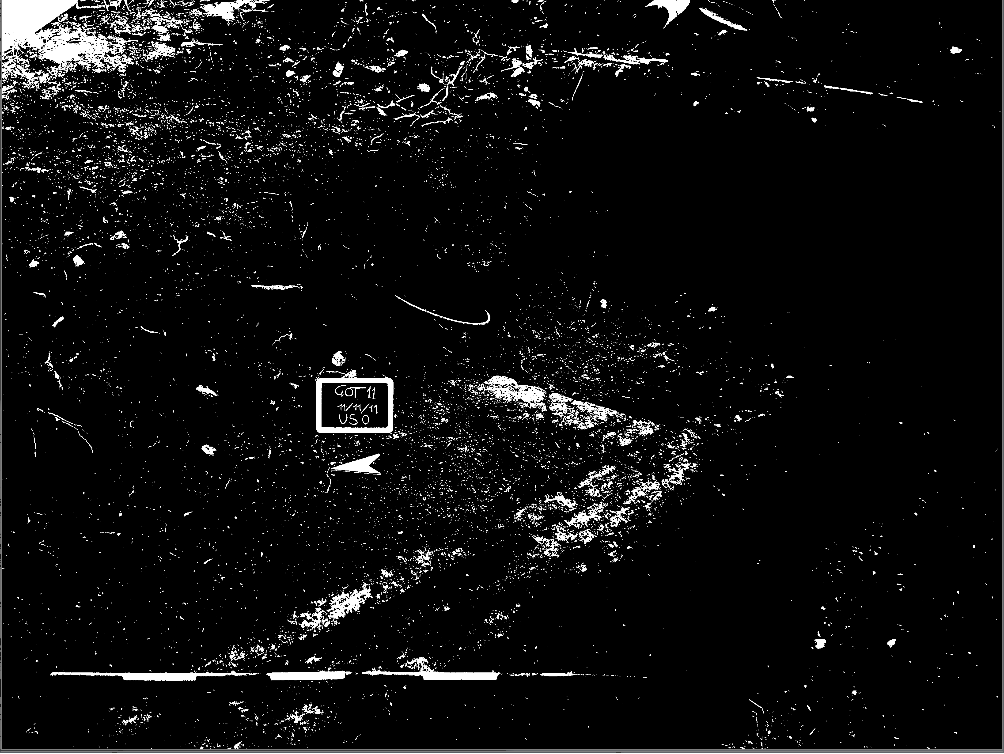
\includegraphics[width =0.5\textwidth]{thresh185.png}
\caption{Grabungsfoto im Original (o.l.), mit niedrigem (60, o.r.), mittlerem (125, u.l.) und hohem (185, u.r.) Schwellwert.}
\label{fig:threshold}
\end{figure}
Daher wurde für den ersten Ansatz ein adaptiver Threshold \cite{opencvadaptivethreshold}) gewählt: Statt global, über das gesamte Bild, einen Schwellwert festzulegen, können lokale Schwellwerte errechnet werden. Die Größe des lokalen Ausschnittes sowie das exakte Verfahren können dabei frei gewählt werden. %In diesem Fall wird für die Binarisierung ein Gauss-Verfahren auf einen Kernel von 11 x 11 Pixeln angewendet.
In diesem Fall wurde für die Binarisierung ein Kernel von 11 x 11 Pixeln angewendet: Für jeden Pixel im Bild wurde durch die Kreuzkorrelation mit dem Gaußfenster die gewichtete Summe der Pixel innerhalb des Kernels berechnet, um diese als lokalen Schwellwert zu verwenden.
Die Beleuchtung oder Farbunterschiede innerhalb des Bildes konnten so ausgeglichen werden (Abbildung \ref{fig:adaptivethreshold}).

\begin{figure}[h!]
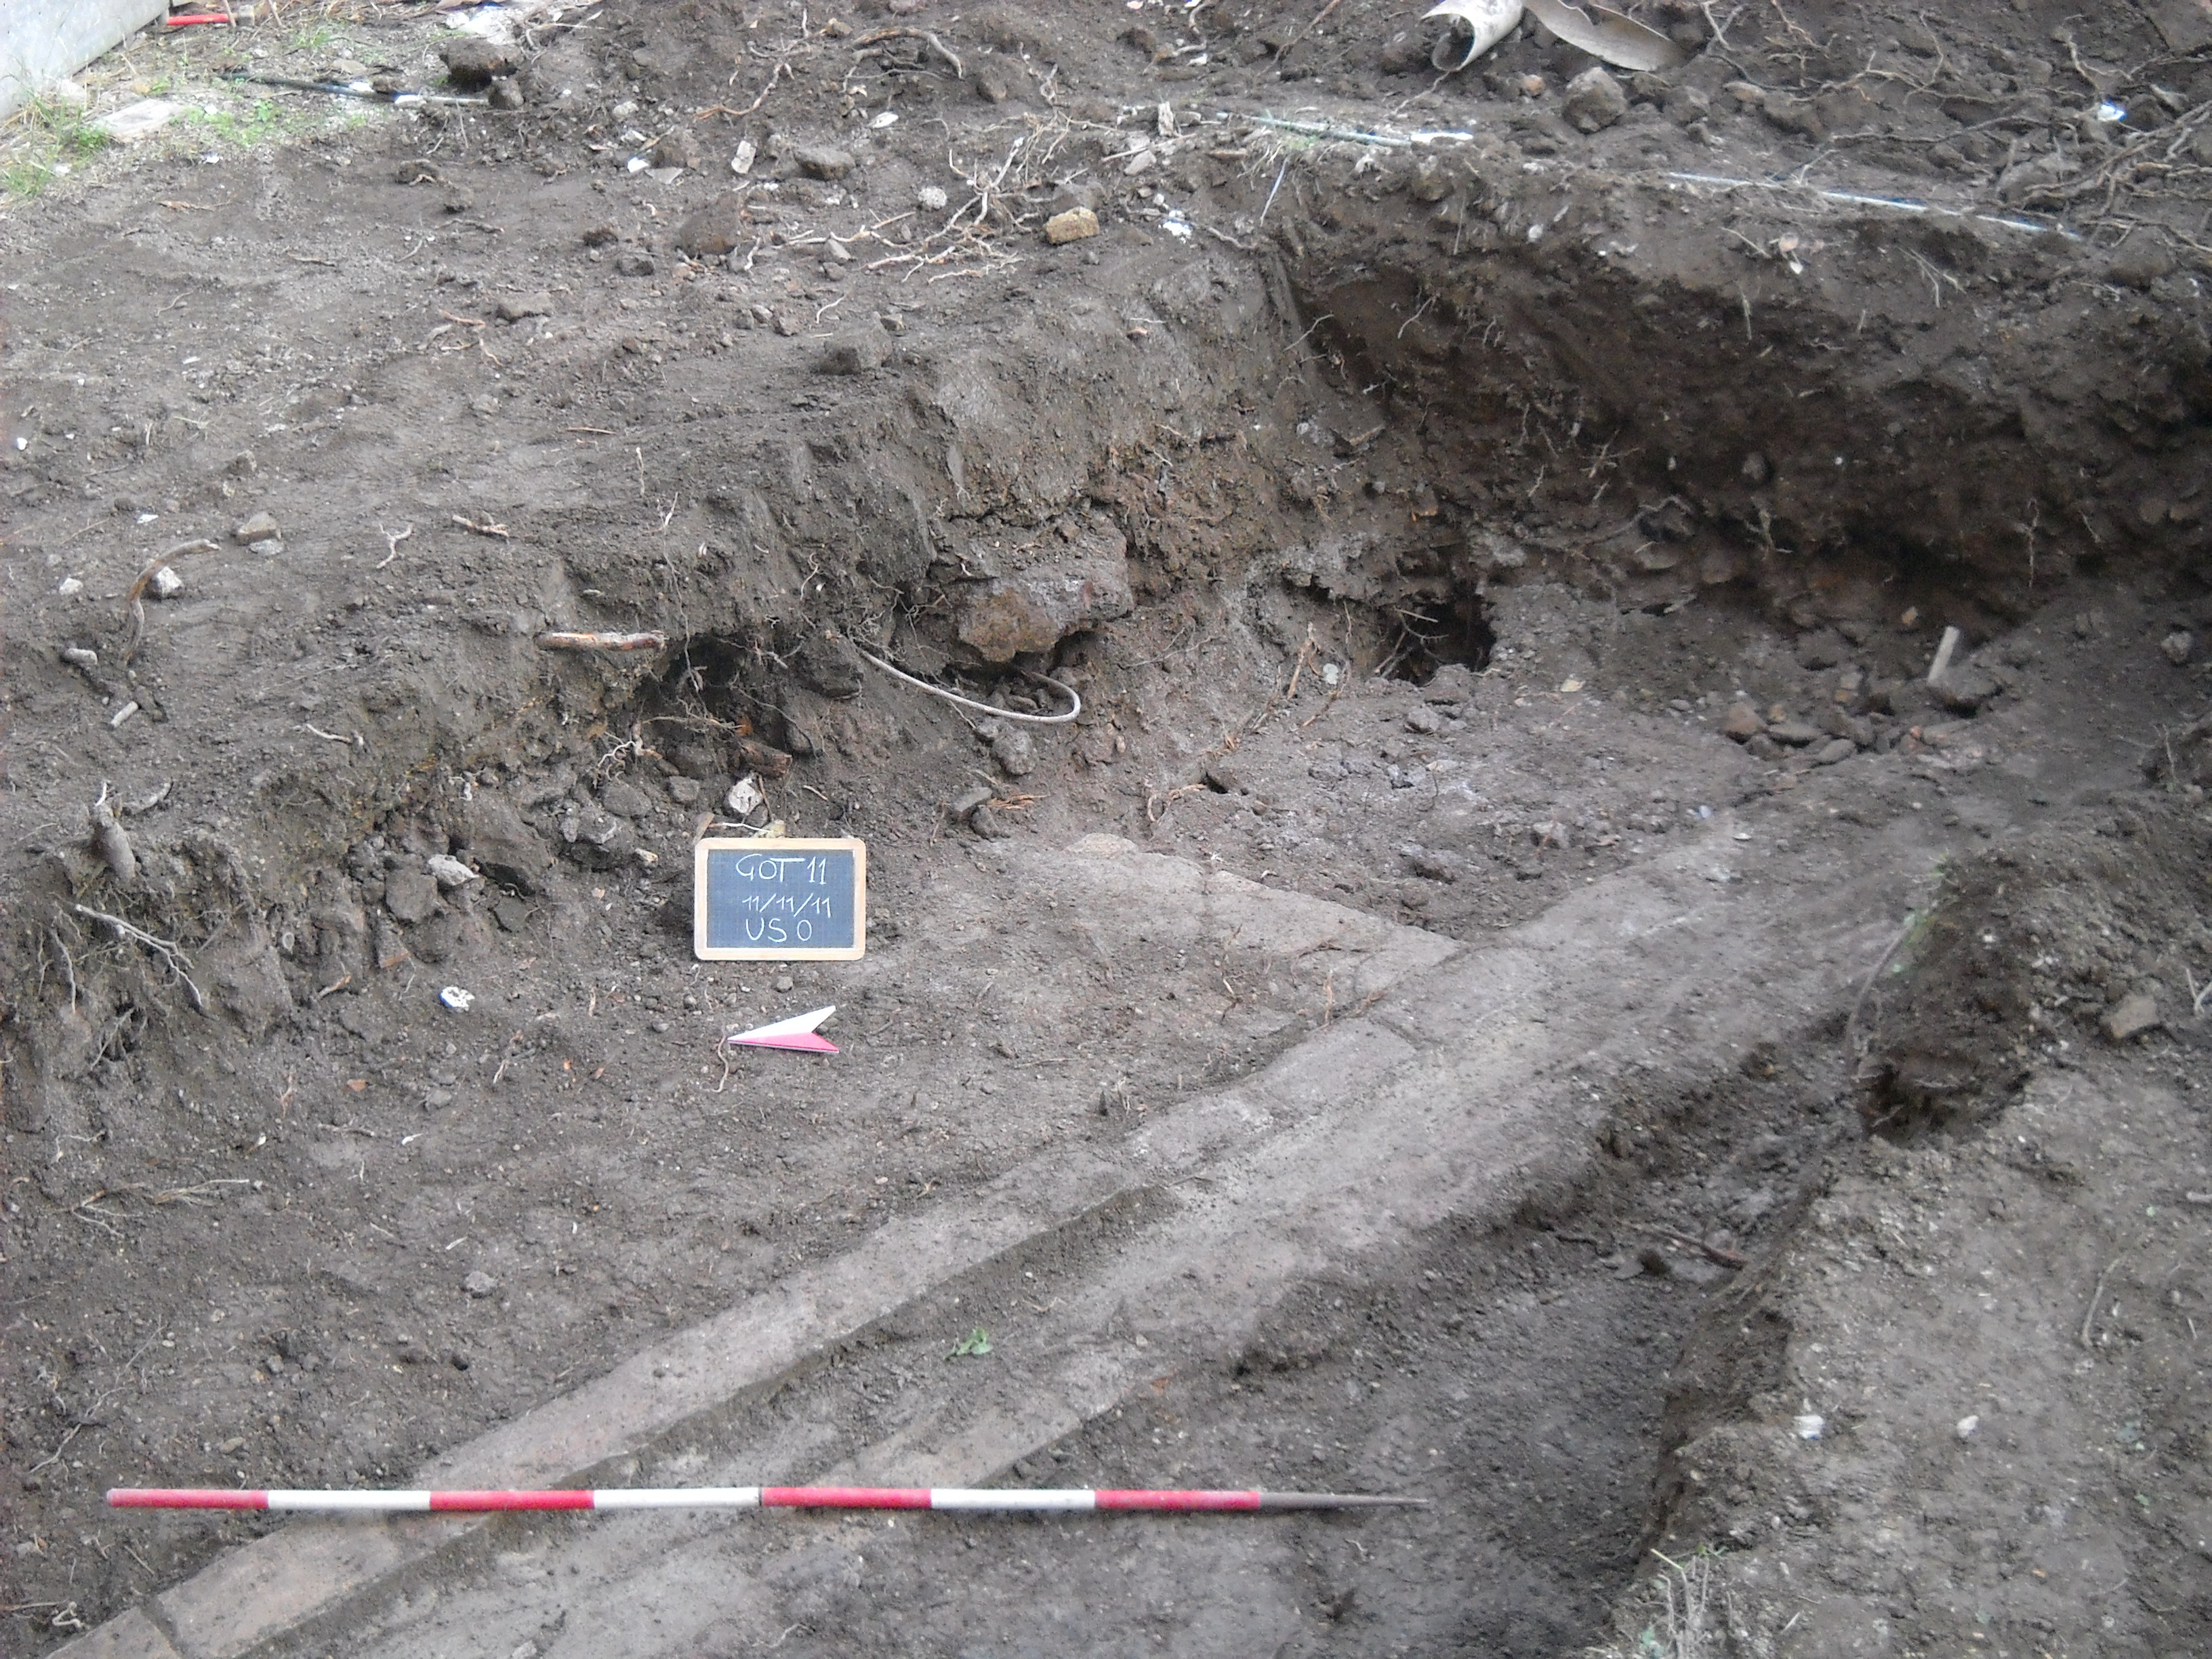
\includegraphics[width =0.5\textwidth]{catacom_1020.JPG}
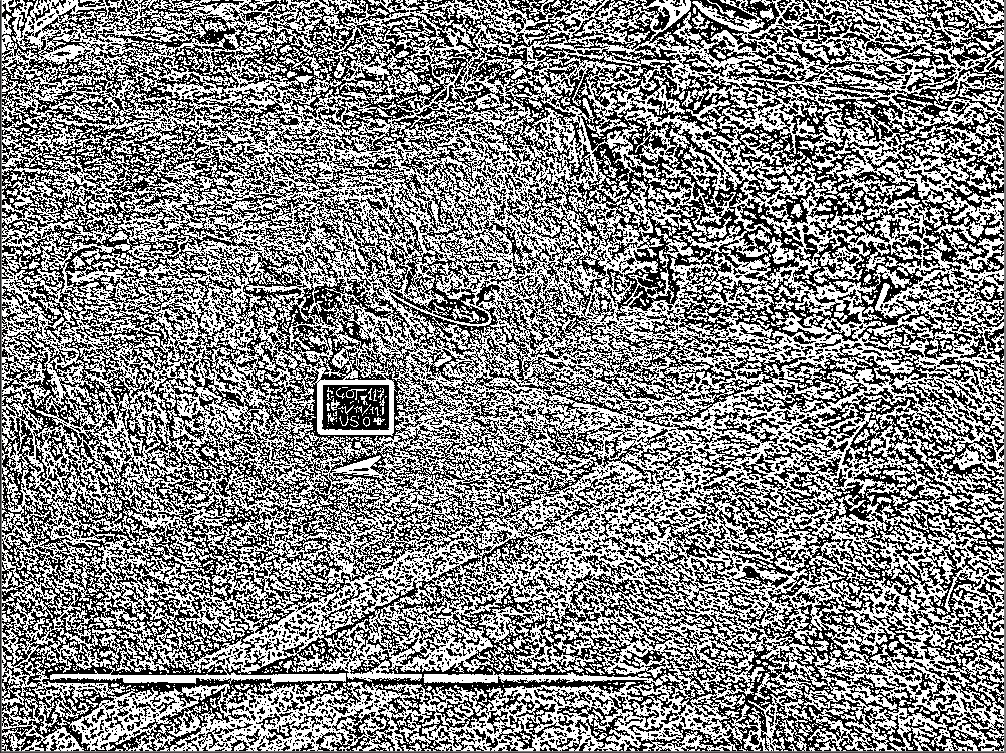
\includegraphics[width =0.5\textwidth]{adaptivethreshold.png}
\caption{Grabungsfoto im Original sowie mit adaptivem Threshold.}
\label{fig:adaptivethreshold}
\end{figure}
Vor der Binarisierung wurde das Bild in ein Graustufenbild umgewandelt und, unter Beibehaltung der Seitenverhältnisse, auf eine Größe von 1000 x 750 Pixeln verkleinert. Das verbesserte die Genauigkeit der Detektion und verringert die zu verarbeitende Datenmenge, wodurch eine Beschleunigung des Prozesses zu erwarten war. %Die Verkleinerung des Bildes ist allerdings ein Prozess, der später rückgängig gemacht werden muss, um Datenverlust bei der Texterkennung zu verhindern.

\subsubsection*{Iterative Binarisierung}

%Die adaptive Binarisierung bringt einige Nachteile mit sich. So ist hier die Erkennung von Falsch-Positiven relativ hoch. Die Konturen werden auf einem verkleinerten Bild gesucht und müssen später auf Originalgröße skaliert werden, was ein verlustbehafteter Prozess ist.
Die Grundidee der iterativen Binarisierung bestand darin, das Bild mit einem globalen Schwellwert zu binarisieren. Dabei ergab sich das Problem, dass bei großen Beleuchtungsunterschieden oder sehr hellen oder dunklen Objekten auf dem Bild ganze Bereiche durch den Schwellwert von der weiteren Bearbeitung ausgeschlossen wurden. Der iterative Ansatz sah daher vor, den Schwellwert von 20 auf 200 in Fünferschritten zu erhöhen. Dadurch entstanden pro Foto 37 binäre Bilder, auf die die Konturenerkennung angewendet werden konnte. Auf jedem dieser Bilder konnten mehrere mögliche Tafeln erkannt werden\footnote{Die eigentliche Tafelerkennung wird erst im folgenden Abschnitt beschrieben. Da die dort gewonnenen Informationen nicht, wie beim adaptiven Ansatz, an das Hauptprogramm übergeben, sondern innerhalb der Funktion des iterativen Ansatzes weiter verarbeitet werden, ist hier ein Vorgriff nötig.}. Der nächste Schritt bestand also darin, aus diesen möglichen Tafeln die auszuwählen, die am wahrscheinlichsten tatsächlich eine war. Dazu wurde eine Grundannahme getroffen: In dem Bereich, in dem auf den meisten der 37 Bilder eine Tafel vermutet wurde, befindet sich tatsächlich eine Tafel. Alle anderen wurden als Falsch-Positive betrachtet. Diese Annahme beruht auf zwei Faktoren: Erstens hat sich gezeigt, dass Objekte, die keine Tafeln sind, aber als solche erkannt werden können -- z.B. Fenster, Türen oder Plakate -- nur unter wenigen Schwellwerten als solche eingeordnet werden. Das liegt unter anderem daran, dass die Tafeln einen hellen Holzrahmen und eine dunkle Innenfläche haben, was zu einem starkem Kontrast führt, der auf vielen Stufen des Schwellwertes erhalten bleibt\footnote{Die Tafeln verfügen damit über eine Eigenschaft, die auch beim Einsatz von AR-Markern genutzt wird: Starke Hell-Dunkel Kontraste beschleunigen und vereinfachen die Detektion [p.~45]{armarker}}. Außerdem wurden durch eben diesen Rahmen in mittleren Schwellwert-Bereichen die Tafeln oft zweimal erkannt: Einmal an der Außenkante und einmal an der Innenkante des Rahmens. Dadurch häufte sich die Detektion möglicher Tafeln in diesem Bereich.\\
Basierend auf dieser Annahme wurde für alle möglichen Tafeln immer paarweise die \verb|intersection over union| berechnet. Dieser Algorithmus basiert auf dem Jaccard-Koeffizienten zur Berechnung der Ähnlichkeit zweier Mengen \cite{intersectionoverunion}. Der Koeffizient wird errechnet, indem die Schnittmenge durch die Vereinigungsmenge geteilt wird. Das Ergebnis liegt zwischen 0 und 1. Je mehr es sich der 1 annähert, desto ähnlicher sind die Mengen. Diese Berechnung lässt sich auch auf die Rechtecke, mit denen die möglichen Tafeln verortet werden, anwenden (Abbildung \ref{fig:jaccard}).

\begin{figure}[h!]
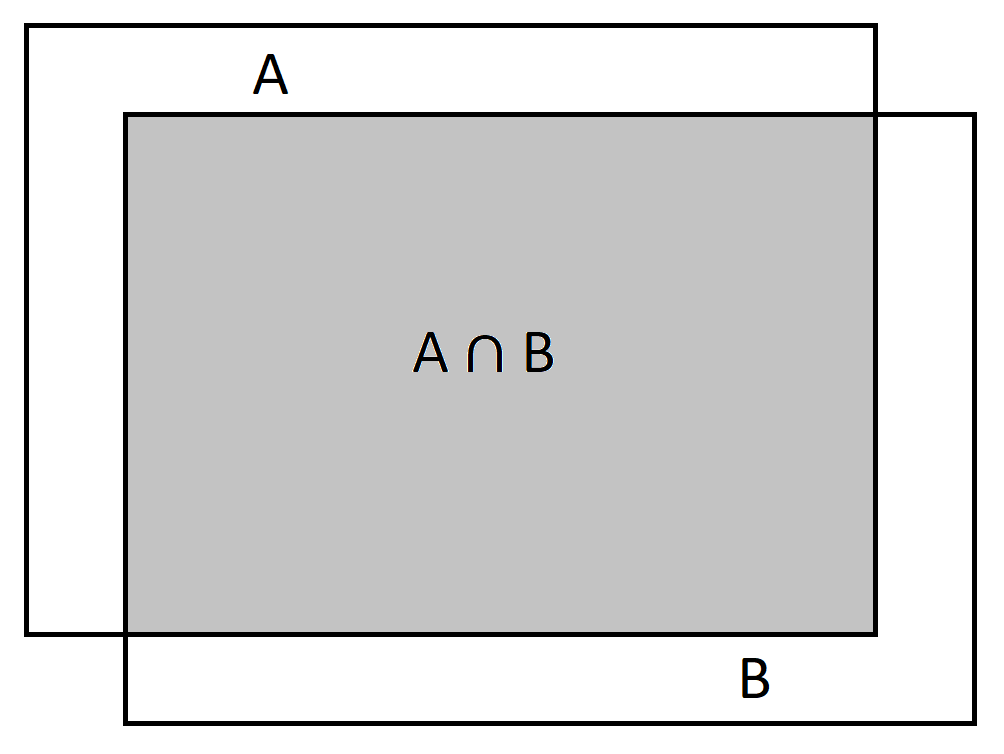
\includegraphics[width =0.5\textwidth]{schnittmenge.png}
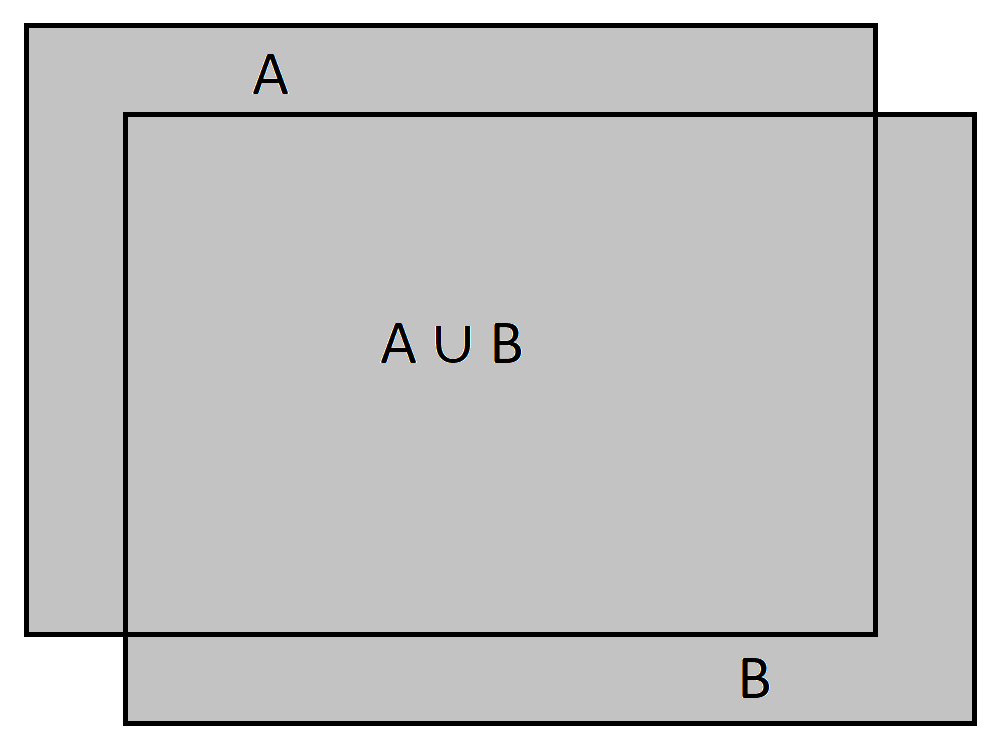
\includegraphics[width =0.5\textwidth]{vereinigungsmenge.png}
\caption{Schnittmenge und Vereinigungsmenge von Rechtecken. Der Jaccard-Koeffizient wird durch die Division der beiden Flächen bestimmt.}
\label{fig:jaccard}
\end{figure}

Zwei Rechtecke gelten im entwickelten Algorithmus dann als hinreichend ähnlich, wenn der Jaccard-Koeffizient über 0.9 liegt. Jedes Mal, wenn ein Rechteck im Vergleich mit einem anderen diesen Wert erzielte, wurde für das Rechteck ein Zähler erhöht. Das Rechteck, welches am Ende der Vergleiche den höchsten Wert in diesem Zähler erzielte, wurde als tatsächliche Tafel angenommen. Eine Ausnahme ergab sich, wenn dieser Wert unter 6 lag. In diesem Falle wurde von Falsch-Positiven und somit einem Foto ohne Tafel ausgegangen. %Je höher der Wert, desto sicherer ist die Identifikation der Tafel. Unter guten Bedingungen erreicht er Werte um die 20.

\subsubsection*{Rechteckserkennung}

War die Binarisierung der Bilder nach einer der beiden vorgestellten Methoden erfolgt, konnten mittels \verb|cv2.findContours| die Konturen der Objekte darauf gefunden werden (Abbildung \ref{fig:adaptivecont}). Die Hierarchie der Konturen wurde dabei außer Acht gelassen, da sich daraus keine verlässlichen Informationen gewinnen ließen.
\begin{figure}[h!]
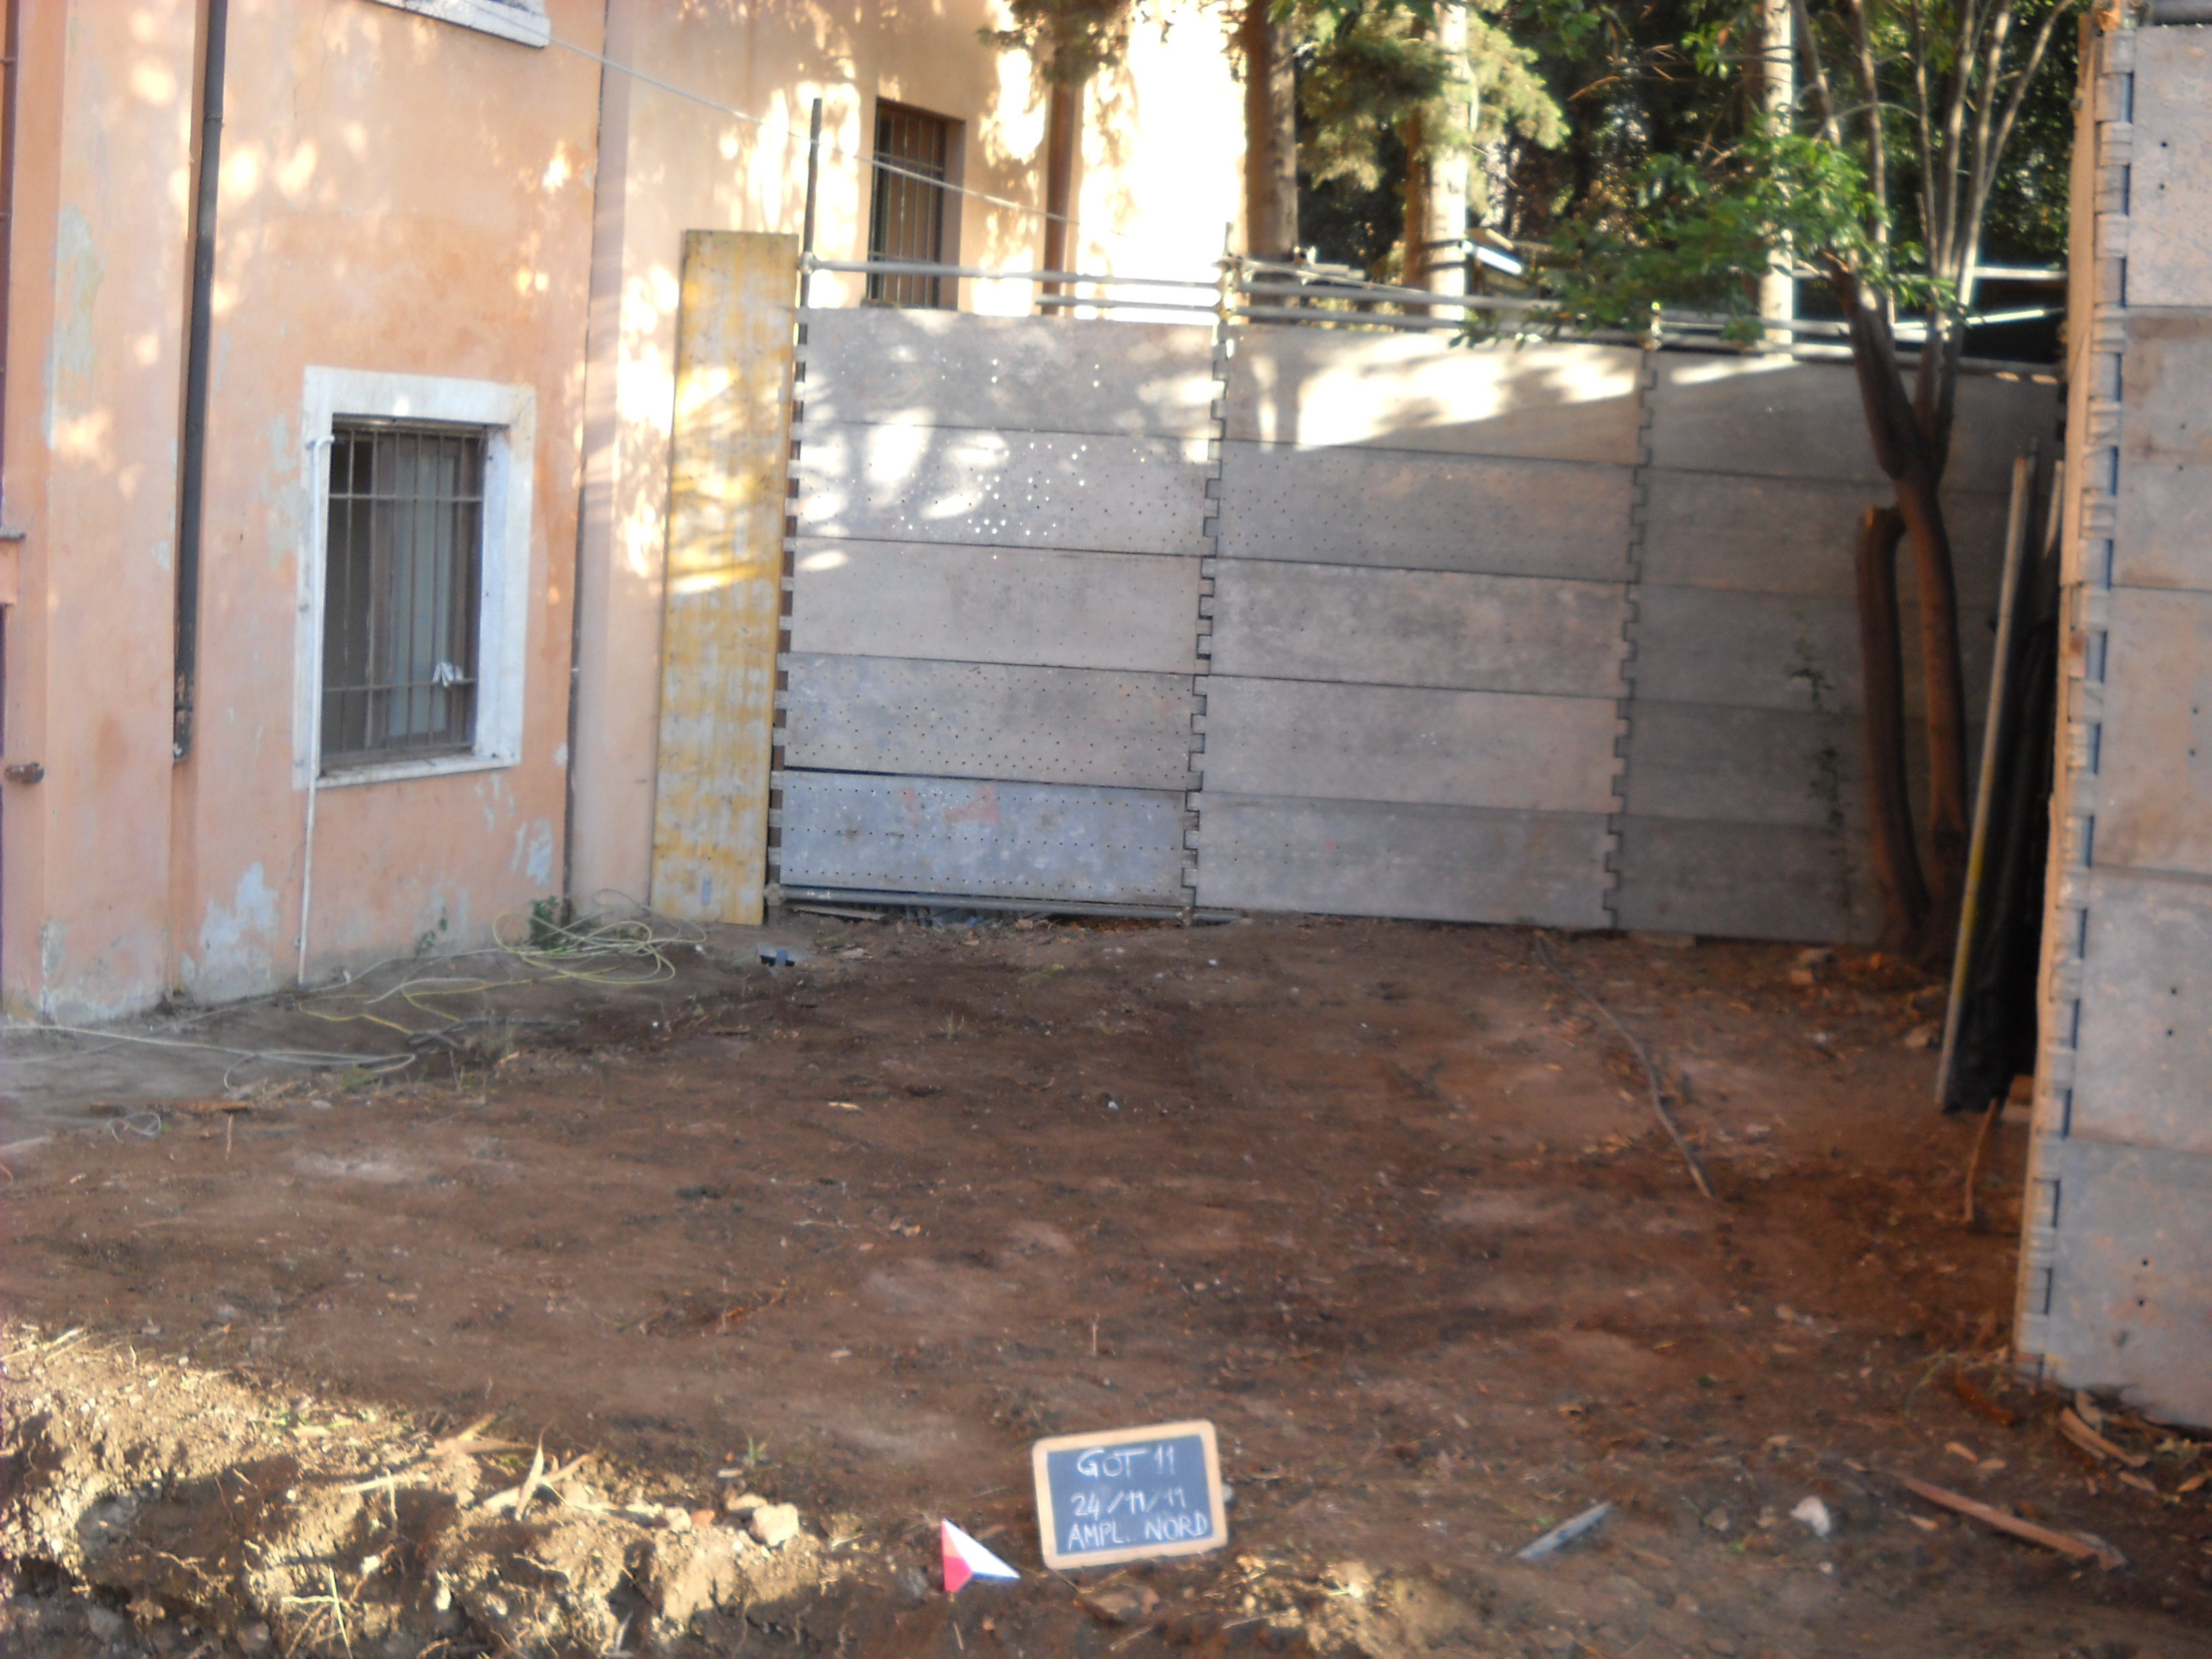
\includegraphics[width =0.5\textwidth]{catacom_1111.JPG}
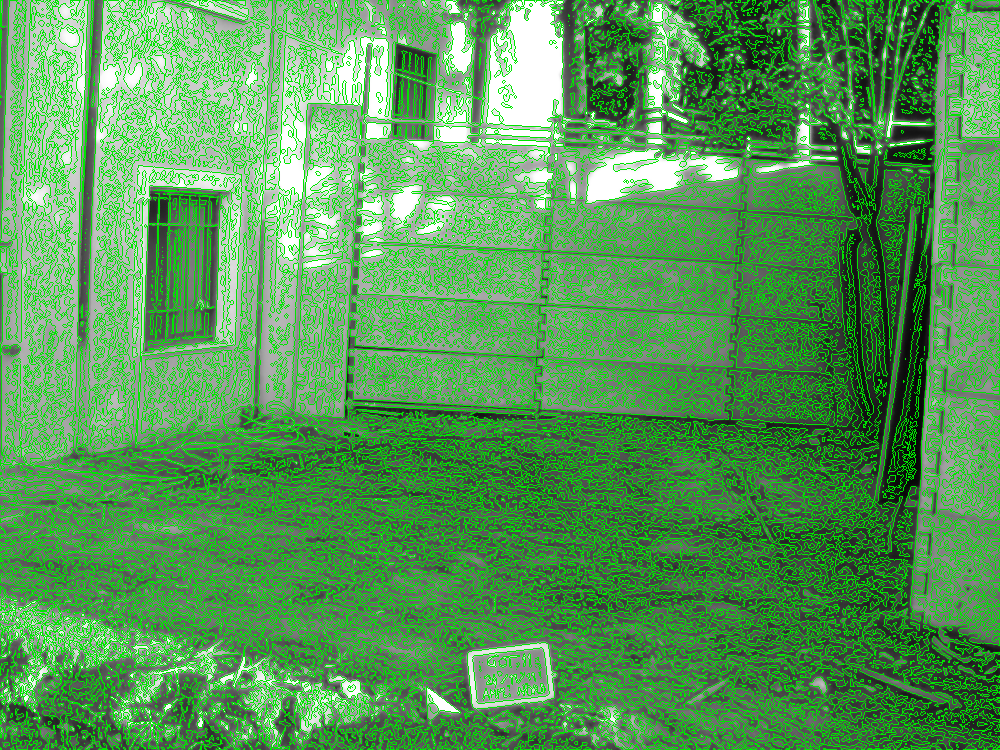
\includegraphics[width =0.5\textwidth]{catacom_1111_adaptive_cont.png}
\caption{Grabungsfoto im Original sowie nach der Anwendung der Konturerkennung.}
\label{fig:adaptivecont}
\end{figure}
%Zweispurigkeit der Ansätze: iterativ und adaptiv. Erklären warum.
%\verb|rect_detect| als Finale, in dem die beiden Ansätze wieder zusammengeführt werden
Als nächstes mussten unter diesen Konturen die ausgewählt werden, die als Tafel in Frage kamen. Dazu wurde die Tatsache genutzt, dass Tafeln auf den Fotos zumindest annähernd als Rechtecke abgebildet werden. Durch ihre Lage zur Kamera können sie zu einem gewissen Grad davon abweichen, grundsätzlich bleibt diese Form aber erhalten. Andere Rechtecke kommen zwar vor, wie Plakate, Fenster, Türen, Ziegel und Fliesen, unterscheiden sich jedoch meist in der tatsächlichen Form oder können im Zweifelsfall bei der späteren Texterkennung ausgeschlossen werden. Dementsprechend ging es in der weiteren Tafelerkennung darum, Rechtecke zu finden und diese durch verschiedene weitere Kriterien so zu sortieren, dass alle Tafeln und möglichst nur Tafeln erkannt werden. Das wurde in mehreren Schritten erreicht:
Zunächst wurde die Fläche der Konturen berechnet. Genutzt wurde hierfür die OpenCV-Funktion \verb|cv2.contourArea|. War die Fläche zu klein, wurde die Kontur aussortiert. Als Maß wurde hier die Kantenlänge der längsten Kante des Bildes genommen, damit bei höherer Auflösung weiterhin korrekt sortiert werden konnte (Abbildung \ref{fig:adaptivecontsize}). Eine Größenbegrenzung ist sinnvoll, da die Tafeln in der Regel eher prominent im Bild zu sehen sind. Sollte tatsächlich eine Tafel durch dieses Kriterium aussortiert werden, wäre die spätere Texterkennung ohnehin so erschwert, dass die Tafel in der weiteren Verarbeitung keinen Mehrwert hätte.
\begin{figure}[h!]
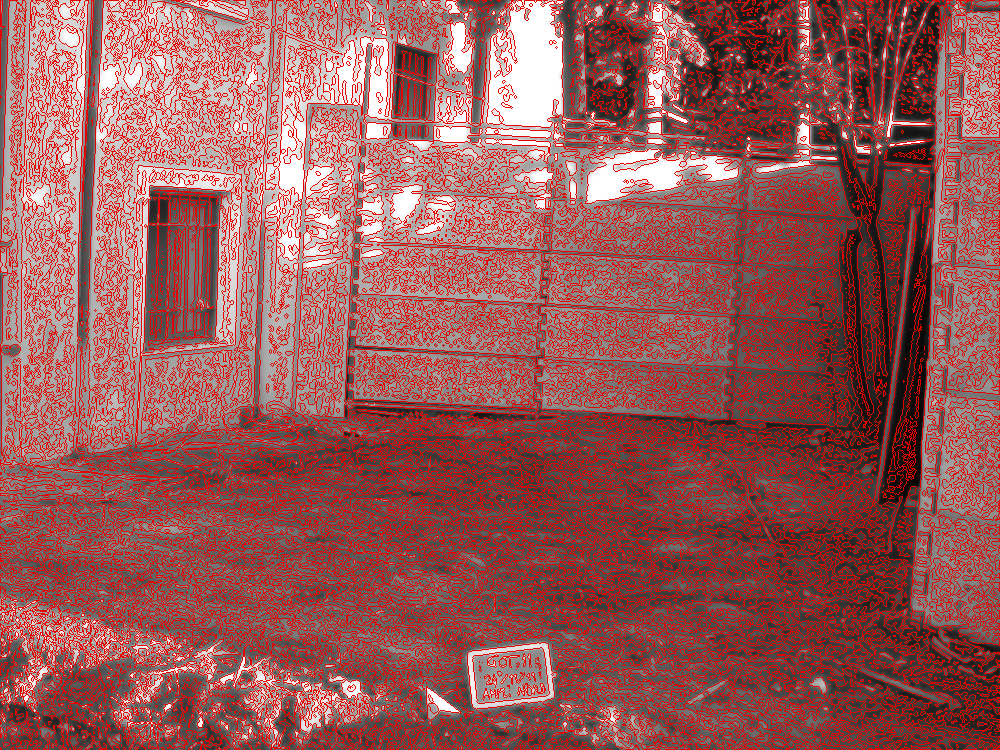
\includegraphics[width =0.5\textwidth]{catacom_1111_adaptive_contred.png}
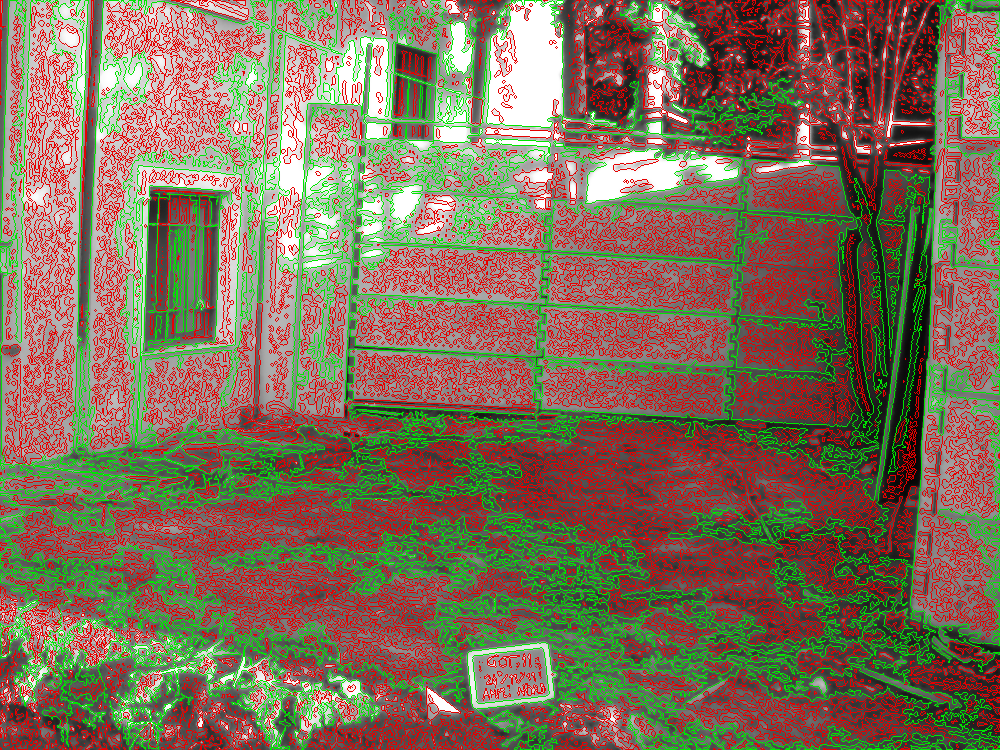
\includegraphics[width =0.5\textwidth]{catacom_1111_adaptive_bigcont.png}
\caption{Konturen vor und nach der Selektion nach Fläche.}
\label{fig:adaptivecontsize}
\end{figure}

Der nächste Schritt bestand darin, durch \verb|cv2.minAreaRect| das kleinstmögliche Rechteck um die Kontur zu bilden (Abbildung \ref{fig:adaptiverectangles}).
\begin{figure}[h!]
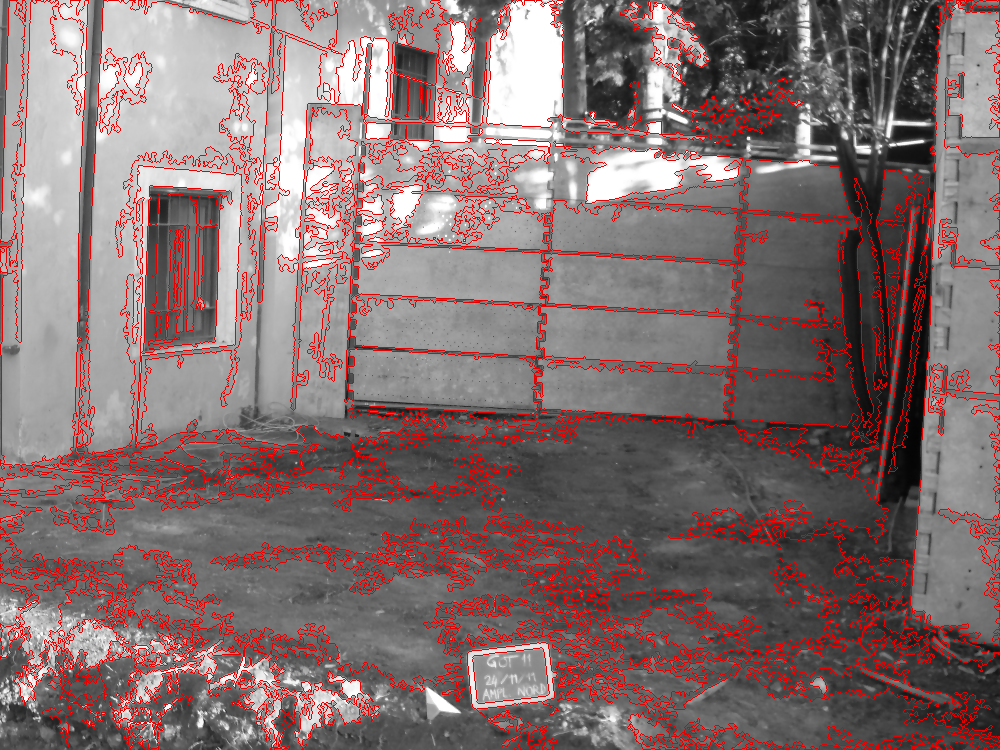
\includegraphics[width =0.5\textwidth]{catacom_1111_adaptive_bigcontred.png}
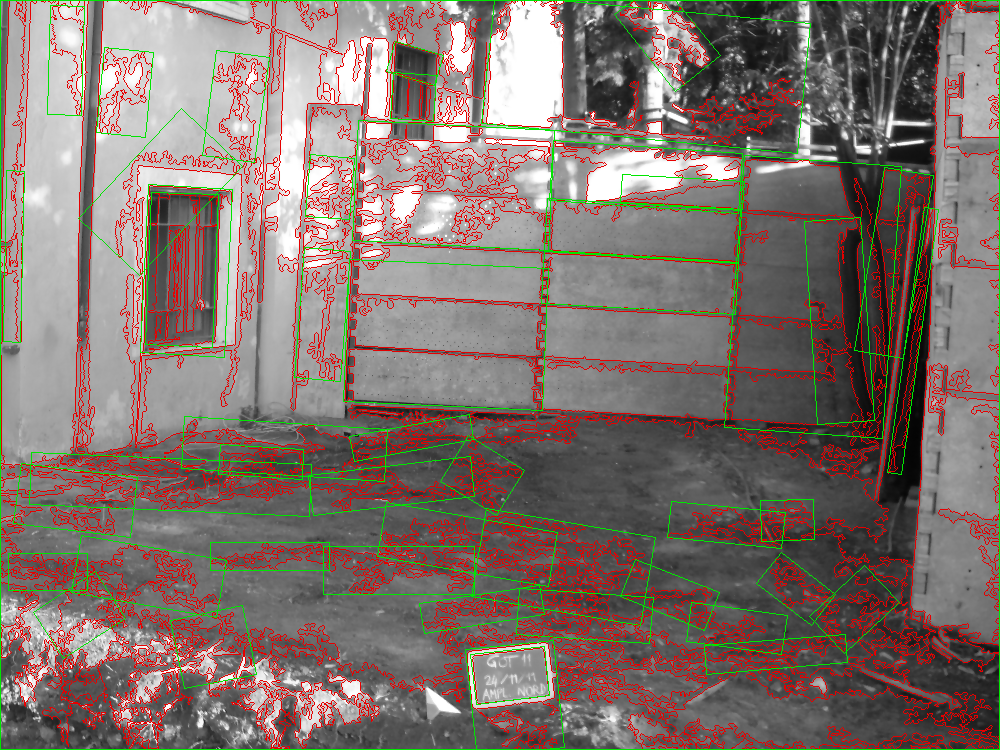
\includegraphics[width =0.5\textwidth]{catacom_1111_adaptive_allrects.png}
\caption{Konturen ohne und mit Rechtecken.}
\label{fig:adaptiverectangles}
\end{figure}

Anschließend wurden die bereits berechneten Flächen der Konturen mit denen der kleinstmöglichen Rechtecke verglichen. Die Annahme: Nähert sich der Flächeninhalt der Kontur dem des Rechtecks an, handelt es sich bei der Kontur selbst wahrscheinlich um ein Rechteck. Dabei hatte sich als Schwellwert bewährt, dass die Fläche der Kontur 85\% der Fläche des Rechtecks betragen sollte. Ebenfalls ausgeschlossen wurde ein Rechteck, wenn es die Fläche des gesamten Bildes ausmachte, da teilweise, wie auch bei diesem Beispiel, der Rand des Bildes als Kontur erkannt werden kann (Abbildung \ref{fig:adaptivrect}).
\begin{figure}[h!]
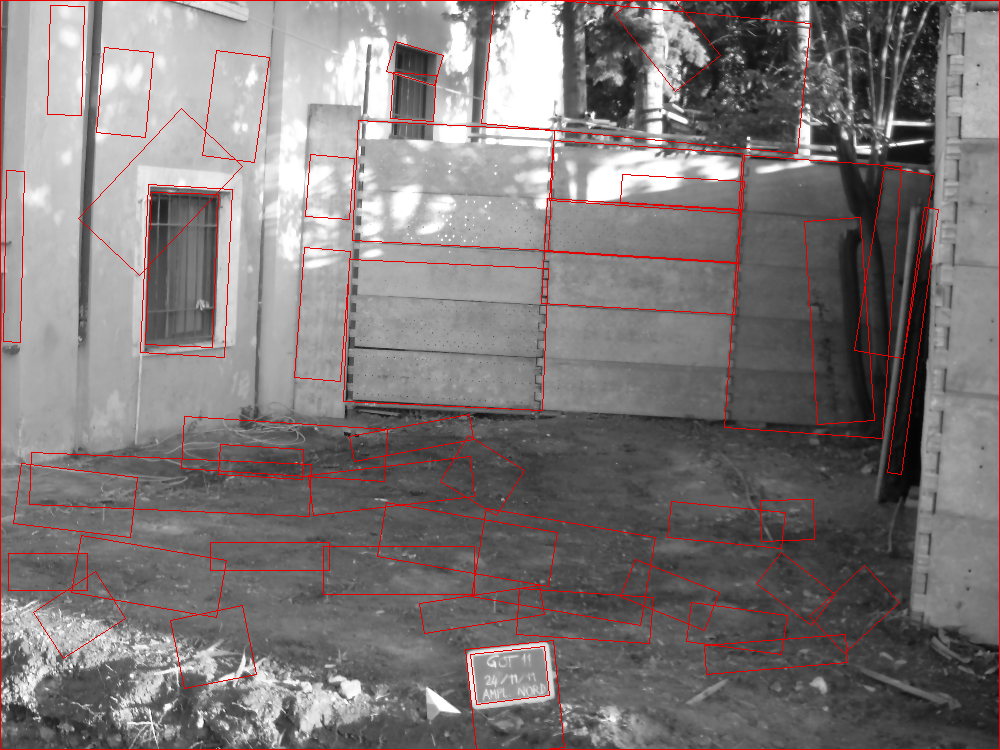
\includegraphics[width =0.5\textwidth]{catacom_1111_adaptive_allrectsred.png}
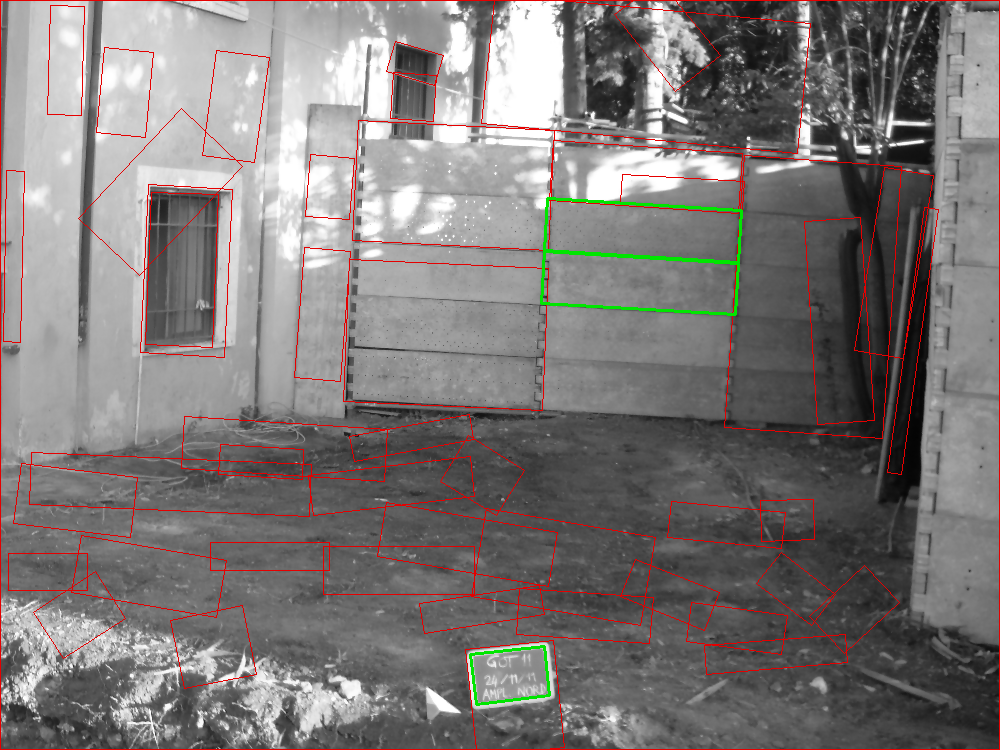
\includegraphics[width =0.5\textwidth]{catacom_1111_adaptive_rectarea.png}
\caption{Rechtecke aller Konturen und jene derer mit annähernd rechteckiger Fläche.}
\label{fig:adaptivrect}
\end{figure}

Als letztes Kriterium wurde das Seitenverhältnis herangezogen. Im Programm besteht die Möglichkeit, vor der Untersuchung aller Bilder ein Template zu hinterlegen, auf dem eine Tafel gut und eindeutig zu sehen ist. Aus diesem Template wurde das Seitenverhältnis der Tafel berechnet. Findet dieser Schritt nicht statt, wird ein maximales Seitenverhältnis von 2:1 angenommen, da Tafeln selten in länglichen Formaten zu finden sind\footnote{Sollte das Format einer Tafel doch einmal von dieser Annahme abweichen, lassen sich hier problemlos Anpassungen vornehmen.}. Mit einer deutlichen Toleranz von 30\% in jede Richtung wurde das Seitenverhältnis der verbliebenen Rechtecke mit dem des Templates verglichen. Waren die Werte sich ähnlich genug, wurde das Rechteck als Tafel interpretiert und galt als das Ergebnis des Algorithmus (Abbildung \ref{fig:aspectratio}).
\begin{figure}[h!]
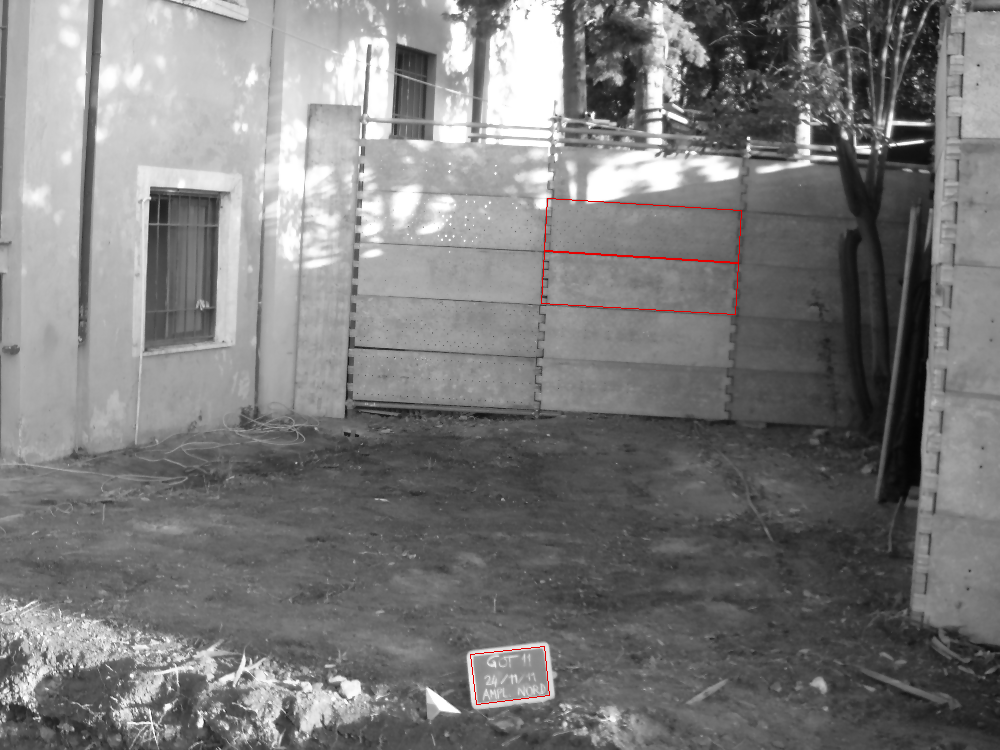
\includegraphics[width =0.5\textwidth]{catacom_1111_adaptive_rectareared.png}
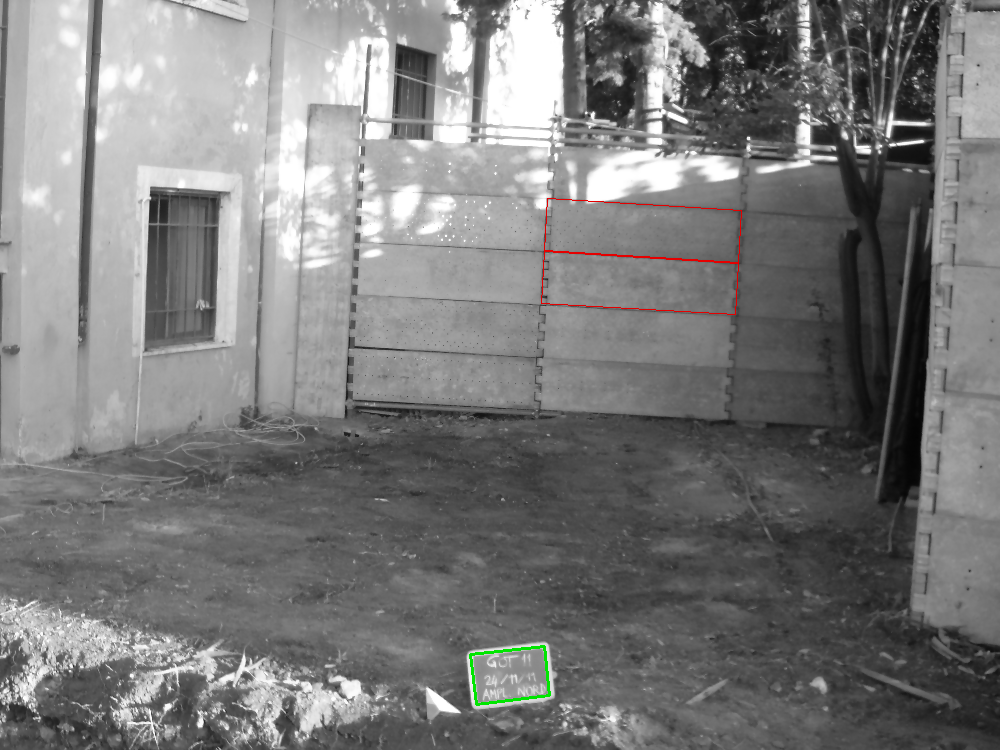
\includegraphics[width =0.5\textwidth]{catacom_1111_adaptive_aspectratio.png}
\caption{Die bisher verbliebenen Rechtecke und die mit dem richtigen Seitenverhältnis.}
\label{fig:aspectratio}
\end{figure}
 
\subsection{Cropverfahren}

Durch die vorhergehende Rechtecksdetektion waren die Positionen der Tafeln bekannt. Der nächste Schritt bestand darin, die Tafeln aus dem Gesamtbild auszuschneiden, damit diese Ausschnitte für die Texterkennung genutzt werden konnten. Auch die perspektivischen Verzerrungen der Tafeln mussten ausgeglichen werden. Für diesen Ausgleich mussten die Eckpunkte der Tafeln bestimmt und das durch sie definierte Viereck auf die Fläche eines Rechtecks übertragen werden.//
Auch hier ergaben sich wieder zwei Verfahren, von denen eines effizient arbeitet, während das zweite stärker auf das Entzerren der Bilder abzielt (Abbildung  \ref{fig:flowchartcrop}).
\begin{figure}[h!]
\centering
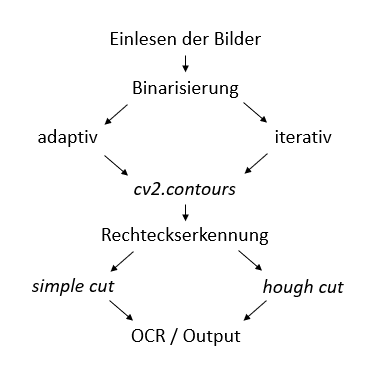
\includegraphics[width =0.5\textwidth]{flowchart_cont_crop.PNG}
\caption{Vollständiges Flowchart, welche Prozesse die Fotos durchlaufen. Nach der Rechteckserkennung schließt sich jetzt eines der beiden Crop-Verfahren an.}
\label{fig:flowchartcrop}
\end{figure}
%Was ist die Aufgabe beim Crop?
%Worin liegen hier die Schwierigkeiten?
%Auch hier wieder Zweispurigkeit der Ansätze erklären

\subsubsection{Simple Crop}

Ein Weg, die Tafeln aus den Bildern auszuschneiden, bestand darin, die kleinstmöglichen Rechtecke aus dem Detektionsverfahren als Basis für den Ausschnitt zu nutzen. Basierte die Detektion auf dem adaptiven Ansatz, musste zunächst das Rechteck auf die ursprüngliche Bildgröße skaliert werden, da für die weitere Verarbeitung die Originalbilder mit der höheren Auflösung verwendet wurden. Zu diesem Zweck wurde das Verhältnis aus der Größe des Originalbildes und der des skalierten Bildes gebildet. Multipliziert man dieses Verhältnis mit den vier Kennzahlen der Rechtecke (X- und Y-Koordinate des Mittelpunktes sowie Breite und Höhe) wird das Rechteck passend skaliert. Als letzter Schritt wurden aus diesen Werten, unter Einbeziehung der Rotation des Rechtecks, die Eckpunkte berechnet.  Neben den so erhaltenen Ausgangskoordinaten mussten aber auch Zielkoordinaten erzeugt werden, auf die das Rechteck projiziert wird. Diese wurden ebenfalls dem Detektionsrechteck entnommen, indem Höhe und Breite als Maße für das Projektionsziel genutzt wurden.\\
Für die Transformation des Ausgangsrechtecks auf das Zielrechteck wurde mittels \verb|cv2.getPerspectiveTransform| die Transformationsmatrix erzeugt (\cite{cvtransform}). Die eigentliche Transformation erfolgte dann durch \verb|cv2.warpPerspective| (Abbildung  \ref{fig:aspectratio}).\\
Der so erzeugte Tafelausschnitt wurde anschließend auf 1000 Pixel skaliert, was in der Regel eine Vergrößerung darstellt, um eine einheitliche Größe zu gewährleisten und zu kleine Ausschnitte zu vermeiden. Außerdem wurde das Bild um 90 \degree rotiert, wenn die Höhe die Breite übertraf, um nur Ausschnitte im Querformat zu erhalten.

\begin{figure}[h!]
\centering
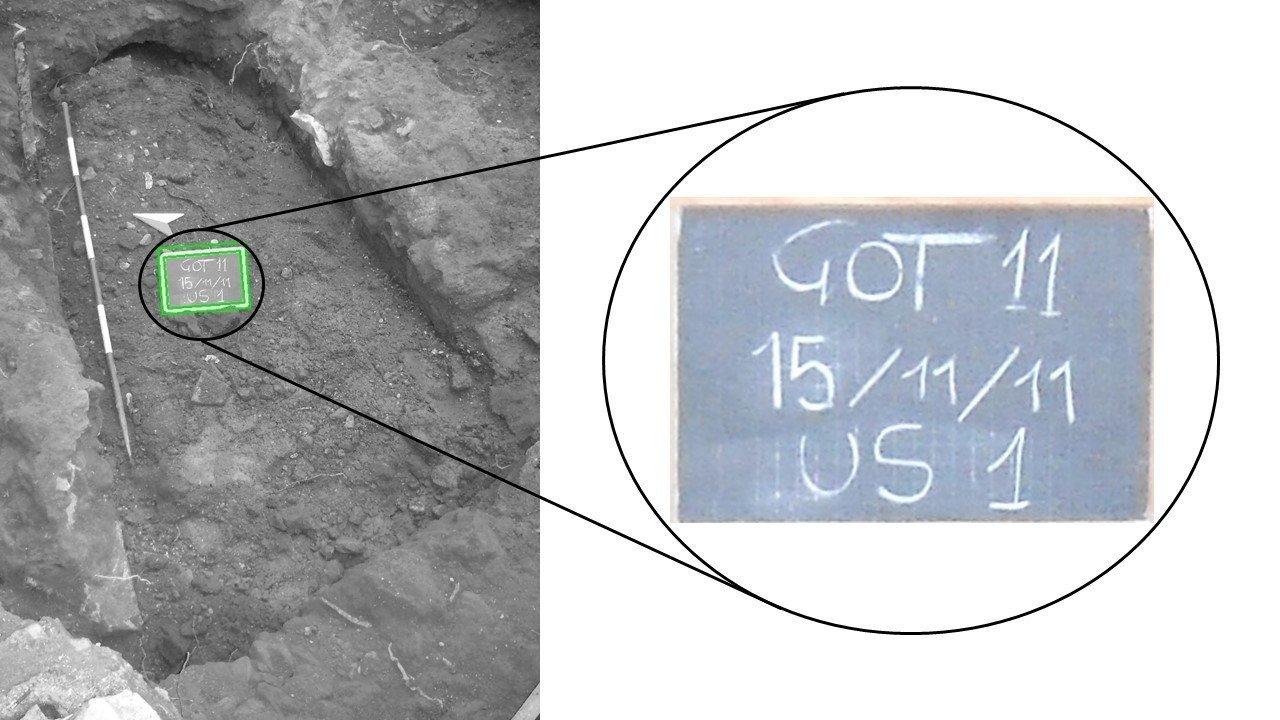
\includegraphics[width =0.75\textwidth]{Tafel Zoom.jpg}
\caption{Eine Tafel vor und nach dem Ausschneiden.}
\label{fig:tafelcrop}
\end{figure}

\subsubsection{Hough\protect\footnote{Gesprochen: [h\textturnv{}f]} Crop}

%Was ist die Idee?
%Wie wurde sie umgesetzt?
%Wo liegen die Probleme?
Durch die unterschiedlichen Perspektiven, aus denen die Fotos aufgenommen wurden, ist die beschriftete Seite der Tafeln nicht immer frontal der Kamera zugewendet. \verb|Simple Crop| ist nicht geeignet, um die daraus resultierende Verzerrung auszugleichen (Abbildung  \ref{fig:parallelogramm}). 

\begin{figure}[h!]
\centering
\includegraphics[width =0.5\textwidth]{catacom_1073_simple.png}
\caption{Diskrepanz zwischen den Eckpunkten der gefundenen Rechtecke und den Eckpunkten der Tafel.}
\label{fig:parallelogramm}
\end{figure}

Daher wurde ein zweiter Ansatz entwickelt, um dieses Problem zu beheben. Ziel war es hier, statt der Eckpunkte der gefundenen Rechtecke die Eckpunkte der Tafel für das Cropverfahren zu nutzen. Diese mussten also zunächst gefunden werden. Das kann erreicht werden, indem die Seiten der Tafeln durch Kantendetektion ermittelt und im Anschluss deren Schnittpunkte berechnet werden \cite{qixiangye}{} \cite{shaw}.\\
Zunächst musste dazu ein passender Bildausschnitt gewählt werden. Auf den Tafeln befinden sich viele Objekte, die lange gerade Kanten aufweisen. Nach der Detektion zu entscheiden, welche davon Teil einer Tafel sind und welche nicht, ist komplex und würde die gesamte Problematik der Detektion neu aufwerfen. Gleichzeitig konnten auch die detektierten Rechtecke nicht verwendet werden, da hier Teile des Rahmens abgeschnitten sein können. Daher wurde das zu schneidende Gebiet um den Faktor 1,3 vergrößert und mittels \verb|simple crop| ausgeschnitten (Abbildung \ref{fig:tafelrechteck}.

\begin{figure}[h!]
\centering
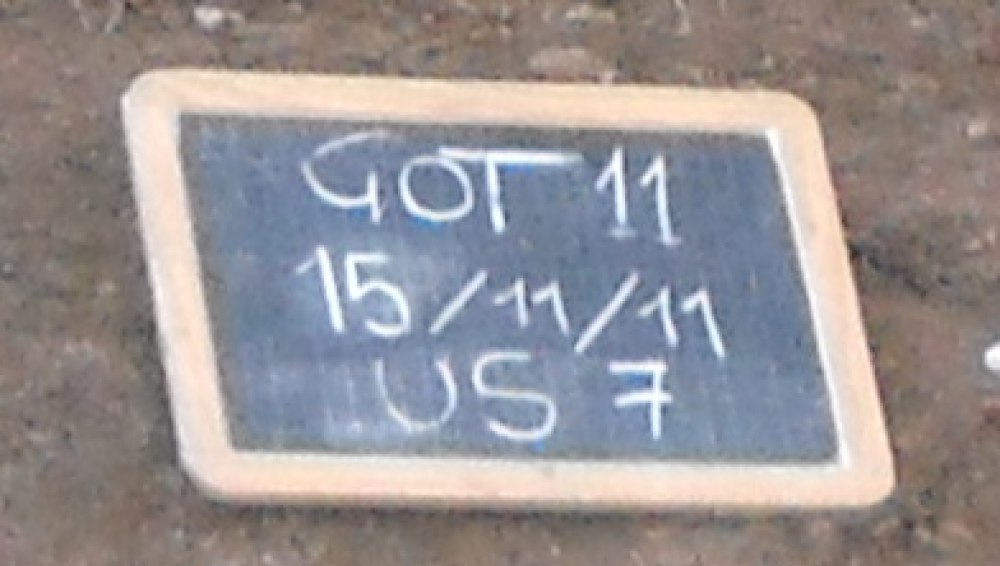
\includegraphics[width =0.5\textwidth]{1073_new_rect.png}
\caption{Bildausschnitt für Hough Crop, basierend auf dem vergrößerten Tafelrechteck.}
\label{fig:tafelrechteck}
\end{figure}

Diese Bildausschnitte wurden mit mehreren Filtern bearbeitet, um das meist stark vorhandene Rauschen zu reduzieren. Es folgte die Umwandlung in ein Graustufenbild, das normalisiert wurde. Beim Prozess der Normalisierung werden Farbskalen, in diesem Fall die Graustufen, auf ihre maximalen Werte gestreckt. Der niedrigste wird auf 0, der höchste auf 255 gesetzt und alle Werte dazwischen werden entsprechend angepasst (Abbildung \ref{fig:norm}).

\begin{figure}[h!]
\centering
\includegraphics[width =0.5\textwidth]{1073_norm.png}
\caption{Graustufenbild, gefiltert und normalisiert.}
\label{fig:norm}
\end{figure}

Auf die normalisierten Bilder wurde die \textit{Canny Edge Detection} (Kantenerkennung) angewendet \cite{cannyedge}. Dieser Algorithmus berechnet die Gradienten der einzelnen Pixel, wodurch Kantenverläufe im Bild erkennbar werden. Auf diese wird eine \textit{non-maximum supression} angewendet, d.h., die Gradienten der Pixel werden mit ihren Nachbarn verglichen und jeweils nur das Maximum weiterverwendet. Die Kantenstärke wird somit auf die Breite von einem Pixel reduziert. Aus den so erhaltenen Gradienten werden mittels zweier Schwellwerte durch Hysterese die gewünschten Kanten bestimmt. Das bedeutet:  Enthält ein Pixel einer Kante den zweiten, höheren Schwellwert, gilt sie als eine der gesuchten Kanten. Von dort ausgehend werden alle Pixel der Kante, die den niedrigeren Schwellwert übertreffen, ebenfalls Teil dieser Kante (Abbildung \ref{fig:canny}).
\begin{figure}[h!]
\centering
\includegraphics[width =0.5\textwidth]{1073_canny.png}
\caption{Kantendetektion mit dem Canny-Algorithmus.}
\label{fig:canny}
\end{figure}

Dieses Gradientenbild wurde anschließend mittels Hough-Transformation \cite{houghpatent}{} einer Linienerkennung unterzogen. Die vorher detektierten Kanten, die einen beliebigen Verlauf nehmen können, wurden jetzt darauf geprüft, ob sie eine gerade Linie bilden. Dazu wird mit der hesseschen Normalform jede mögliche Gerade durch jeden Kantenpunkt berechnet. Jedes Kantenpixel, durch das die Geraden verlaufen, erhält einen \textit{upvote}, es wird also ein Zähler inkrementiert. Durch die Bereiche mit den meisten \textit{Upvotes} laufen die gesuchten Linien auf dem Bild. Ist eine Linie gefunden, ist sie wahrscheinlich Teil des Rahmens der Tafel und somit für die Erkennung der Eckpunkte relevant (Abbildung \ref{fig:lines}.
\begin{figure}[h!]
\centering
\includegraphics[width =0.5\textwidth]{1073_lines.png}
\caption{Linienerkennung mit dem Hough-Algorithmus.}
\label{fig:lines}
\end{figure}

Im nächsten Schritt wurden die Geraden mit dem Bildrahmen geschnitten. Die Schnittpunkte wurden als neue Endpunkte des Liniensegments für die weiteren Berechnungen genutzt, um etwaige Schnittpunkte außerhalb des Bildes ausschließen zu können. Die Endpunkte wurden, entsprechend ihrer Position im Bild, den vier Ecken zugeteilt. Anschließend wurden die Schnittpunkte der Linien untereinander berechnet, aber nur, wenn sie (1) nicht in die gleiche Richtung und (2) nicht diagonal durchs Bild verliefen. Beide Kriterien konnten durch die Einordnung der Eckpunkte bestimmt werden. Damit war sichergestellt, dass nur Linien miteinander geschnitten wurden, die annähernd senkrecht zueinander verlaufen, wie es bei den Tafelrändern der Fall ist. Schnittpunkte am Rand wurden ausgeschlossen, um die Detektion des Bildrandes oder Störobjekte auszuschließen.\\
Die Gruppe der Schnittpunkte wurde in die vier Ecken aufgeteilt. In jeder Ecke wurde dann der Punkt bestimmt, der am weitesten Richtung Bildmitte liegt. Dieser wurde als der wahrscheinlichste Eckpunkt angenommen (Abbildung \ref{fig:intersection}).
\begin{figure}[h!]
\centering
\includegraphics[width =0.5\textwidth]{1073_intersection.png}
\caption{Die Schnittpunkte der Linien nach der Berechnung. Die roten Punkte liegen zu nahe am Rand und wurden daher ausgeschlossen.}
\label{fig:intersection}
\end{figure}
Das weitere Verfahren entsprach dem des \verb|simple crop|-Ansatzes: Mit den Eckpunkten wurde eine Transformationsmatrix berechnet, durch die der Bildausschnitt innerhalb der vier Eckpunkte auf eine Rechtecksform übertragen werden konnte (Abbildung \ref{fig:houghcrop}).
\begin{figure}[h!]
\centering
\includegraphics[width =0.5\textwidth]{catacom_1073_hough.png}
\caption{Die Tafel, in ein Rechteck transformiert.}
\label{fig:houghcrop}
\end{figure}

\subsection{Texterkennung}

Im folgenden Abschnitt wird der zweite Aspekt der Verarbeitung von Grabungsfotos vorgestellt: Die Texterkennung oder \textit{optical character recognition}. Da die Vorbereitung der Bilder für das Gesamtergebnis von großer Bedeutung ist, wird zunächst das \textit{Preprocessing} behandelt. Im Anschluss wird die eigentliche Texterkennung mit Tesseract vorgestellt.\\
Folgende Probleme müssen bei der Texterkennung adressiert werden: (1) Komplexität der Szene\footnote{Gemeint ist hier, wie komplex die Szene ist, wenn das Foto in einer natürlichen Umgebung aufgenommen wurde. Text auf einer das Bild füllenden Hauswand zu finden ist weniger anspruchsvoll als die Detektion von Text in einer Straßenszene mit Häusern, Autos und Pflanzen.}, (2) Beleuchtungsverhältnisse, (3) Rotation des Textes relativ zur Kamera, (4) Unschärfe, (5) Größe und Format der Textfelder, (6) Neigungswinkel des Textes relativ zur Kamera, (7) Schriftart, (8) Mehrsprachigkeit, (9) perspektivische Verzerrungen \cite{hamad}. In diesem Falle wurde allen Aspekten, die der Textdetektion gelten (1, 5), geringeres Gewicht beigemessen, da die Tafeln bereits als die Grenzen des beschriebenen Areals betrachtet werden konnten. Die Neigung und die Schiefe der Buchstaben relativ zur Kamera (3, 6, 9) wurden bereits beim Cropverfahren entsprechend den Möglichkeiten ausgeglichen. Beleuchtung, Unschärfe und Rauschen waren Teil des Preprocessings (2, 4), die sprachbezogenen Punkte (7, 8) wurden im Rahmen der eigentlichen Texterkennung adressiert.

\subsubsection{Preprocessing}

Das Preprocessing für die Texterkennung folgte gängigen Verfahren\footnote{Weitere übliche Schritte im Preprocessing, wie das Thresholding, unterblieben hier. Die Gründe dafür werden im Kapitel \ref{section:diskussiontexterkennung} diskutiert.} \cite{jenilshah}{}  \cite{sumedhahallale}. Zunächst mussten die Bilder in Graustufen umgewandelt werden. Nacheinander wurden zwei Filter angewendet, \verb|cv2.GaussianBlur| \cite{opencvfilter}{} und \verb|cv2.fastNlMeansDenoising| \cite{opencvdenoise}. Ersterer dient als Weichzeichner, Letzterer reduziert das Rauschen, indem Pixel verschoben werden, die dem Farbwert nach nicht in ihre Umgebung passen. Damit sollten die Störeffekte durch verwischte Kreide auf der Tafel reduziert werden. Das Bild wurde invertiert, sodass die eigentliche weiße Kreide schwarz dargestellt und der Hintergrund hell wurde, was den Empfehlungen für Tesseract entspricht \cite{tesseractoptimum}. Der letzte Schritt bestand in der Normalisierung der Bilder. Alle diese Schritte wurden auf das Grundbild sowie jeweils auf die daraus extrahierten 3 Farbkanäle angewendet \cite{xilinchen}.

\subsubsection{OCR}

Pro gefundener Tafel waren jetzt vier Bilder vorhanden, die der Texterkennung unterzogen werden konnten. Für jedes Bild wurde diese zweifach ausgeführt: Einmal mit \verb|image_to_string| und einmal mit \verb|image_to_boxes|. Ersteres liest den Text zeilenweise ein und versucht dabei, ganze Wörter zu erkennen, Letzteres liest jeden Buchstaben einzeln, wodurch die Ergebnisse variieren. \verb|Image_to_string| wurde zusätzlich auf das um 180\degree{} rotierte Bild angewendet, um die Orientierung zu ermitteln: Die Ergebnisse der Texterkennung beider Orientierungen wurden, nach der Bereinigung von Leerzeichen und Zeilenumbrüchen, anhand der Länge miteinander verglichen. Die Version, bei der mehr Text gefunden wurde, wurde als korrekt orientiert angenommen\footnote{Alternative wäre hier die Verwendung der \textit{confidence} möglich gewesen, also der Wert, mit dem angegeben wird, für wie wahrscheinlich ein Neuronales Netz die angegebene Kategorisierung angibt, also wie sicher es bei diesem Ergebnis ist. Dieser Wert kann nicht bei allen Tesseract-Funktionen erhoben werden und wurde daher hier ausgeschlossen.}. Diese Annahme folgt daraus, dass die Texterkennung unter erschwerten Bedingungen stattfindet und Buchstaben oft nicht erkannt werden. Werden also mehr Buchstaben erkannt, kann davon ausgegangen werden, dass die Erkennung insgesamt besser ist. Eine solche Funktion ist zwar in Tesseract bereits grundsätzlich implementiert, da die Texterkennung aber ohnehin unter erschwerten Bedingungen und ohne erkennbare Wörter stattfand, wurde hier ein eigener Ansatz verwendet\footnote{U.a. liefert die Funktion image\_to\_osd von Pytesseract die Orientierung des gefundenen Textes; für dessen Anwendung befindet sich auf den Tafeln jedoch zu wenig Text.}.
Die Ergebnisse der beiden Pytesseract-Funktionen aus den je vier Bildern wurden im Anschluss untereinander verglichen. Der längste gefundene Text wurde als Ergebnis übernommen.
Beide Befehle wurden mit folgender Konfiguration ausgeführt: (1) Es wurde eine Whitelist verwendet, die auf das Schema der Tafeln zugeschnitten wurde. Gelistet wurden die Ziffern \textit{0-9}, die Buchstaben \textit{G,O,T,U} und \textit{S} sowie das Sonderzeichen \textit{/}. (2) Als Sprache wurde ein eigenes Wörterbuch angegeben, das entsprechend der Tafeln nur wenige Wörter enthält (\textit{US, GOT}. (3) Der \textit{OCR Engine Mode} (oem) wurde auf ein Neurales Netzwerk mit \textit{Long Short-term Memory} \cite{hochreitersepp}{} festgelegt. (4) Für die \textit{Page Segmentation} (psm) wurde ein vollautomatischer Modus, ohne weitere Vorgaben, gewählt. Dabei handelt es sich jeweils um die Standardeinstellungen.

%\subsection{Experimentelles}

%\subsection{Zusammenfassung}
%evtl zusammenfassen wie vorgegangen wurde, warum dieser Weg gut ist und was das Wichtigste Ergebnis ist
\subsection{Evaluation}

Die Ergebnisse sowohl bei Tafelerkennung und -ausschnitt als auch bei der Texterkennung wurden durch statistische Analyse des erkannten Textes evaluiert. Dazu wurden die Texte auf einer Auswahl von 79 Tafeln transkribiert und in einer Liste abgelegt. Dabei handelt es sich um alle Tafeln aus dem Datensatz der Grabung 2011. In diesem Teildatensatz ist eine ausreichend große Vielfalt von Fotos mit und ohne Tafeln enthalten, um den gesamten Prozess bewerten zu können. Fotos, auf denen die Tafeln nur teilweise zu sehen sind, wurden hier als Fotos ohne Tafeln gewertet. Die Liste wurde dann als Referenz (Grundwahrheit) für die Auswertung der erkannten Texte eingelesen.\\
Als Maße für die Genauigkeit der Erkennung wurden die Maße \textit{F-Score},  \textit{Recall} und \textit{Precision} verwendet \cite{haraldklinke}{} \cite{qixiangye}. \textit{Recall} gibt dabei an, wie viele der Tafeln tatsächlich erkannt wurden:\\ \begin{equation}Recall = \frac{True Positives}{True Positives + False Negatives}\end{equation}\\Die \textit{Precision} gibt an, wie viele der erkannten Tafeln tatsächlich Tafeln sind:\\\begin{equation}Precision = \frac{True Positives}{True Positives + False Positives}\end{equation}\\Der F-Score erzeugt einen gewichteten, harmonischen Mittelwert aus diesen beiden Maßen, um die Qualität der Tafelerkennung in einem Wert zusammenzufassen:\\\begin{equation}F = 2 \times \frac{precision \times recall}{precision + recall}\end{equation}\\%Der F-Score wurde dabei als bevorzugtes Maß verwendet, die beiden anderen können optional mit ausgegeben werden.
%Aus den F-Scores wurden mehrere Durchschnittswerte gebildet, um das Gesamtergebnis zu evaluieren: (1) Der Mittelwert der zeilenweisen Erkennung, (2) der Mittelwert der buchstabenweisen Erkennung, (3) der Mittelwert aus diesen beiden Werten, (4) der Mittelwert der als bestes Ergebnis eines Bildes ermittelten Textzeilen.
Für die Evaluation der Texterkennung wurde das \verb|ratio| der Funktion \verb|sequence matcher| verwendet, das ein Maß für die Ähnlichkeit zweier Textsequenzen berechnet. Es berechnet sich aus \cite{difflib}:\\
\begin{equation}ratio = 2 \times \frac{Matches}{Length of both Sequences}\end{equation} \\
Durch den stärkeren Einbezug der Länge der Sequenzen schneidet ein Text mit zu vielen erkannten Zeichen in der Tendenz schlechter ab als bei der Berechnung des \textit{F-Scores}, was hier angemessen erschien. Der \textit{F-Score} kann jedoch optional verwendet werden.
\section{Ergebnisse}

In diesem Kapitel werden die Ergebnisse der zuvor vorgestellten Methoden präsentiert. Dabei wird zunächst das Gesamtergebnis präsentiert. Im Anschluss wird auf Besonderheiten bei Tafel- und Texterkennung eingegangen. Basis der Auswertung ist dabei ein Testdatensatz aus 292 Bildern, worunter sich 79 Bildern mit Tafeln befinden.
Im Anschluss werden Versuche mit den Datensätzen anderer Projekte präsentiert.

%Gesamtergebnis mit Genauigkeiten bei Box, Text und insgesamt
\subsection{Gesamtergebnis}
Für das Gesamtergebnis wurden die Tafelausschnitte in den vier Varianten gemeinsam der Texterkennung unterzogen (Vgl. collection.csv). Der durchschnittliche  \textit{F-Score} (\textit{average}) betrug im Ergebnis 0.49. Die Durchschnittswerte der zeilenweisen (\textit{textaverage}) und buchstabenweisen (\textit{boxaverage}) Texterkennung lagen bei 0.51 bzw. 0.47. Die durch das Programm als bestes Ergebnis ausgewählten Zeichenketten (\textit{bestaverage}) erzielten einen \textit{F-Score} von 0.61. Das theoretische Optimum (\textit{optimum}), also der Durchschnitt der tatsächlichen besten Ergebnisse pro Bild, lag bei 0.7. Einige der Tafelausschnitte konnten nicht ausgelesen werden. Das schlechteste Ergebnis wurde bei catacom\_1110 erzielt, auf dem Text nur bei einem von 5 Ausschnitten erkannt wurde (\textit{F-Score} 0.15). Das beste Ergebnis war ein \textit{F-Score} von 1 bei catacom\_1152.\\
\\

\begin{tabular}[h]{c|c|c|c|c|c}
Verfahren & boxaverage & textaverage & average & bestguess & optimum \\
\hline
Gesamt & 0.47 & 0.51 & 0.49 & 0.61 & 0.7 \\
Adaptive Hough & 0.43 & 0.47 & 0.45 & 0.49 & 0.56\\
Adaptive Simple & 0.52 & 0.57 & 0.54 & 0.61 & 0.64\\
Iterative Hough & 0.44 & 0.47 & 0.45 & 0.47 & 0.52\\
Iterative Simple & 0.51 & 0.56 & 0.54 & 0.57 & 0.6\\
\end{tabular}

\subsection{Tafelerkennung}
%recall, precision und f-score für die Tafelfindung
Bei der Tafelerkennung zeigten beide Ansätze gute Ergebnisse, die nur in Nuancen voneinander abwichen.
So erkannte der adaptive Ansatz aus 292 Bildern 133 mit Tafeln. Dass diese Zahl über der der 79 Tafeln lag, ist darin begründet, dass der äußere und der innere Tafelrand Tafel identifiziert werden können, es also bis zu zwei richtige Erkennungen pro Bild geben kann \footnote{Der Einfluss dieses Umstandes auf die Kennwerte ist so gering, dass er vernachlässigbar ist.}. Zudem wurden 8 Falsch-Positive erkannt, Falsch-Negative gab es keine. Der \textit{Recall} lag damit, wie gewünscht, bei 1. Die \textit{Precision} betrug 0.926, der \textit{F-Score} damit 0.961.
Beim iterativen Ansatz wurden 85 Tafeln erkannt. Da dieser Ansatz nur das wahrscheinlichste Ergebnis pro Bild ausgibt und hier keine Falsch-Negativen auftraten, lag die Zahl der Falsch-Positiven bei 6. Der \textit{Recall} war also auch hier 1, die \textit{Precision} 0.929. Der \textit{F-Score} betrug 0.963.
Die relativ hohe Zahl der Falsch-Positiven resultierte aus vier Fotos, auf denen Plakate abgebildet waren. Da Plakate alle Kriterien der Tafeln erfüllen -- rechteckig, passendes Seitenverhältnis, mit Text beschrieben -- konnte der Algorithmus weder in diesem Schritt noch später, bei der Texterkennung, diese Bilder aussortieren. Eine manuelle Entfernung der Bilder aus dem Datensatz, die sich auch in der Praxis als erster Schritt empfehlen würde, steigerte den \textit{F-Score} auf 0.992 beim adaptiven und auf 0.987 beim iterativen Ansatz. Die Unterschiede zwischen beiden Ansätzen sind also gering, wobei die Anfälligkeit für Falsch-Positive im iterativen Ansatz etwas niedriger ist. 
%Adaptiver Ansatz: 292 Bilder input, 133 output, davon 8 Fp und 0 FN, Rest dementsprechend TP. recall = 1, precision = 0.926, f = 0.961 -> Mehr TP als Bilder mit Tafeln, bedingt durch das Verfahren, Einfluss auf statistische Auswertung aber gering
%Iterativer Ansatz: 292 Bilder input, 85 output, davon 6 fp und 0 fn. recall =1, precision = 0.929, f = 0.963
%Fehler vor allem durch Bild mit Plakat. Ohne diese Bilder (1081,1082,1083,1084):
%Adaptiver Ansatz: 292 Bilder input, 127 output, davon 2 Fp und 0 FN, Rest dementsprechend TP. recall = 1, precision = 0.984, f = 0.992
%Iterativer Ansatz: 292 Bilder input, 81 output, davon 2 fp und 0 fn. recall =1, precision = 0.975, f = 0.987
%-> Adaptiver Ansatz insgesamt etwas besser, iterativer etwas robuster, insgesamt aber Unterschiede zu vernachlässigen

%Tafelrkennung: Unterschied zwischen adpativem und iterativen Threshold
Bei der Auswertung der Texterkennung nach Detektionsverfahren ergaben sich Unterschiede: Beim adaptiven Verfahren (ausgewertet mit beiden Schnittverfahren) lag das \textit{bestaverage} des \textit{F-Scores} bei 0.59, das theoretische Optimum bei 0.67 (Vgl. adaptive only.csv). Das iterative Verfahren kam auf einen \textit{F-Score} von 0.56 bei einem Optimum von 0.65 (Vgl. iterative only.csv).
%Tafelerkennung: Unterschied zwischen simple und hough crop
Beim nächsten Schritt, dem Schnittverfahren, variierten die Ergebnisse deutlicher. So erzielte das \textit{bestaverage} des \verb|Hough Crop|-Verfahrens (iterativer und adaptiver Ansatz parallel) einen \textit{F-Score} von 0.49, das theoretische Optimum betrug 0.59 (Vgl. hough only.csv). Im Gegensatz dazu lag das \textit{bestaverage} des \verb|Simple Crop| bei 0.62 und somit noch über der Gesamtauswertung. Das theoretische Optimum lag mit 0.67 etwas unter der Gesamtauswertung (Vgl. simple only.csv).
Als Einzelverfahren war die Kombination \verb|Adaptive Simple Crop| am besten, mit einem \textit{bestaverage} von 0.61 und einem theoretischen Optimum von 0.64 (Vgl. crop adaptive simple.csv).\\
\\
\begin{tabular}[h]{c|c|c|c|c|c}
Verfahren & boxaverage & textaverage & average & bestguess & optimum \\
\hline
Gesamt & 0.47 & 0.51 & 0.49 & 0.61 & 0.7 \\
Adaptive (Hough + Simple) & 0.47 & 0.51 & 0.49 & 0.59 & 0.67\\
Iterative (Hough + Simple) & 0.48 & 0.51 & 0.5 & 0.56 & 0.65\\
Hough (Adaptive + Iterative) & 0.43 & 0.47 & 0.45 & 0.49 & 0.59\\
Simple (Adaptive + Iterative) & 0.52 & 0.56 & 0.54 & 0.62 & 0.67\\
\end{tabular} 
%Tafelerkennung: Cont based cut? -> Diskussion
%Tafelerkennung: Ausfilterung der hough crop-Bilder mit Rahmen im Bild -> besseres Ergebnis?

\subsection{Texterkennung}
%Texterkennung: Unterschied zwischen Box und Text
Im Bereich der Texterkennung ließ sich ein Unterschied zwischen \verb|Image to Box|, also der Buchstabenerkennung, und \verb|Image to Text|, der Zeilenerkennung, feststellen. So war der mittlere \textit{F-Score} bei der Buchstabenerkennung um 0.03 bis 0.05 niedriger als bei der Zeilenerkennung (Vgl. collection.csv u.a.). Im Einzelfall variierten die Ergebnisse jedoch stark, sodass die Buchstabenerkennung deutlich bessere Ergebnisse als die Zeilenerkennung liefern kann, was sich positiv auf den \textit{bestguess} auswirkt.
%Texterkennung: Unterschied zwischen Dictioniary und ohne Dictionary
%Texterkennung: Unterschied zwischen Whitelist und ohne Whitelist
Wie bereits vorgestellt wurde für die Texterkennung ein Wörterbuch und eine Whitelist verwendet. In der Auswertung zeigte sich, dass vor allem die Whitelist das Ergebnis signifikant verbessert. Die Anwendung der Texterkennung ohne Wörterbuch, aber mit Whitelist, auf die mit \verb|Adaptive Simple Crop| erzeugten Tafelausschnitte erzielte die gleichen Ergebnisse wie der Durchlauf mit Wörterbuch, also ein \textit{bestaverage} von 0.61 (Vgl. no dic.csv). Wurden sowohl Whitelist als auch Wörterbuch entfernt, sank der durchschnittliche \textit{F-Score} auf 0.26, wobei die Buchstabenerkennung 0.25 erzielte, die Zeilenerkennung nur 0.01 (Vgl. no config no dic.csv). Schaltete man nur das Wörterbuch dazu, verbesserte sich der Wert der Zeilenerkennung auf 0.26 (Vgl. dic only.csv).
%Bestguess erklären und auswerten
%Problem der theroetisch noch höheren Genauigkeit ansprechen (Auswahl durch Länge ungenügend)
Festzustellen war auch, dass die Auswahl des \textit{bestguess} nie zu Ergebnissen unterhalb es Durchschnitts führte, andererseits aber für deutliche Verbesserungen sorgen konnte. Deutlich wurde das in der Gesamtauswertung aller Ansätze, bei der die Differenz zwischen dem durchschnittlichen \textit{F-Score} der beiden Texterkennungsverfahren (0.49) und dem durchschnittlichen \textit{F-Score} des \textit{bestguess} (0.61) 0.12 Punkte betrug. Allerdings bestand auch ein Unterschied von 0.9 zum theoretischen Optimum (0.7) (Vgl. collection.csv).

% Anwendung auf neue Tafeln

\subsection{Weitere Tafeln}

Bei der Anwendung des Algorithmus auf die projektfremden Tafeln der Gruppe Terrestrische Ökohydrologie der FSU Jena sowie der späteren Grabungen am Kapitol durch das Deutsche Archäologische Institut ergaben sich folgende Ergebnisse:
Bei den Tafeln der Ökohydrologie Jena wurde eine Stichprobe aus 40 Fotos mit Tafeln verwendet. Von diesen wurden 9 korrekt erkannt. Auf 16 Fotos wurde fälschlicherweise ein beiliegendes Maßband erkannt\footnote{Hier ist technisch gesehen kein unerwünschtes Ergebnis erzielt worden: Auch das Maßband enthält rechteckige Felder mit passendem Seitenverhältnis und Zahlen darauf.}. Der \textit{Recall} beträgt hier 0.225, die \textit{Precision} 0.36. Der \textit{F-Score} liegt bei 0.277. Diese Ergebnisse wurden mit dem iterativen Verfahren erzielt. Mittels adaptivem Ansatz konnten keine Tafeln ermittelt werden. Die Texterkennung verlief -- abgesehen von Zahlen auf dem Maßband -- ergebnislos.
Aus den Fotografien der Grabungen des DAI wurden 35 Bilder mit Tafeln darauf ausgewählt. Mit dem adaptiven Verfahren wurden 26 Tafeln erkannt, dazu gab es eine Falsch-Positive. Daraus ergab sich ein \textit{Recall} von 0.743, eine \textit{Precision} von 0.963 und ein {F-Score} von 0.838. Das iterative Verfahren erkannte 25 Tafeln ohne Falsch-Positive. Der \textit{Recall} betrug hier 0.714, die \textit{Precision} 1 und der \textit{F-Score} 0.833.
Für die Texterkennung wurde die Whitelist modifiziert, sodass alle Ziffern und alle Großbuchstaben enthalten waren, wie es der Beschriftung der Tafeln entspricht. Der \textit{F-Score} der Zeilenerkennung lag bei 0.86, der der Buchstabenerkennung bei 0.9. Das theoretische Optimum lag bei 0.91. Der \textit{bestguess} lag mit 0.83 deutlich unter diesen Werten.

\section{Diskussion}
%Zusammenfassung Ausgangslage
%Zusammenfassung Vorgehen
%Zusammenfassung Ergebnisse
%Ausblick
%%%%%%%%%%%%%%%%%%%%%%%%%%

\clearpage
%%%%%%%%%%%% Quellen %%%%%%%%%%%%%%
\bibliographystyle{apalike}
\bibliography{quellen}
%%%%%%%%%%%%%%%%%%%%%%%%%%

\end{document}
